\documentclass[a4paper,oneside]{book}
\usepackage{verbatim}
\usepackage{graphicx}
\usepackage{tabularx}
\usepackage{setspace}
\usepackage{amsmath}
\usepackage{amsfonts}
\usepackage[htt]{hyphenat}
\usepackage{url}
\usepackage{pdfpages}
\usepackage{ootools}

\doublespace

% \includeonly{ch03}

\title{A Framework for Text Categorization \\
DRAFT COPY - CONFIDENTIAL \\
DO NOT DISTRIBUTE}
\author{Ken Williams}

% Some custom commands I use
\newcommand{\naive}{Na\"\i ve}
\newcommand{\aicat}{\class{AI::Cat\-e\-gor\-i\-zer}}

\newcommand{\cats}{\mathcal{C}}
\newcommand{\docs}{\mathcal{D}}
\newcommand{\train}{\mathcal{T}^r}
\newcommand{\test}{\mathcal{T}^e}
\newcommand{\func}{\mathcal{K}}

\DeclareMathOperator*{\ArgMax}{ArgMax}
\DeclareMathOperator{\Entr}{H}

\newcommand{\term}[1]{\emph{#1}}

\hyphenation{database data-base}


\begin{document}

\frontmatter

\begin{titlepage}
\begin{center}
      \mbox{}
      \vspace{1in}
      \vfill
      {\huge A Framework for Text Categorization}\\
      \vfill
      \vfill
      A thesis submitted in fulfillment of the requirements for the degree of
      \vfill
      {\Large Master of Engineering (Research)}\\[6pt]
      by\\[6pt]
      {\Large Ken Williams}
      \vfill
      \vfill
      School of Electrical and Information Engineering\\
      The University of Sydney
      \vfill
      \today
      \vspace*{1.5in}
\end{center}
\end{titlepage}

% \maketitle


\chapter{Abstract}

The field of automatic Text Categorization (TC) concerns the creation
of categorizer functions which assign categories from a pre-defined
set of labels to documents based on the documents' content.  The most
successful modern approaches to TC employ Machine Learning to create
these categorizer functions automatically from a training set of
documents similar to the ones in the target application.

Techniques for creating the categorizer functions are the subject of
active research in the Machine Learning and Text Processing academic
communities, and every stage of the process has many variations.
Because of this complexity, the creation of TC applications is usually
a complicated process requiring a great deal of expertise in TC, the
application domain, and software development.

This thesis concerns the creation of an Object-Oriented Application
Framework for Text Categorization.  Frameworks provide a way to
address difficult software engineering problems by encapsulating the
aspects of applications that tend to remain common from one
application to the next, while allowing variation in the aspects that
tend to change.  This allows significant code and design reuse when
building new applications.

Framework design is among the most difficult tasks in software
engineering, and requires a great deal of problem analysis,
architecture design, and product evaluation.  Design Patterns have
grown popular in order to manage the complexities of these aspects and
to facilitate communication among those involved with the
Object-Oriented design of large software systems.  This thesis uses
Design Patterns to examine several of the important internal
relationships among framework classes.

XXX (Will write this last)

\chapter*{Acknowledgments}

I would like to thank Rafael Calvo for his expert supervision of my
thesis, and for giving me the opportunity to pursue this project.  The
rest of the Web Engineering Group---Jae-Moon Lee, Xiaobo Li, Nick
Carroll, and Gosia Mandrela---provided valuable testing and feedback
on \aicat\ and created a quite pleasant research environment.  The
Language Technology group---particularly Casey Whitelaw, Elisabeth
Crawford, and Jon Patrick---was also a good source of feedback and
inspiration.  The Open-Source community provided incentives to write
clean, usable, documented software by their mere existence.  Research
Assistantship funding from the Capital Markets Co-operative Research
Centre provided much-appreciated support for research on the Signal G
corpus.

On a more personal level, I would like Sheri Schechinger for sticking
with me across ten thousand miles of ocean, and the city of Sydney for
being such a great place to spend time.

\chapter*{Preface}

XXX - Rafael says this is too technical in the beginning.

This thesis presents research into design and implementation of a framework
for automatic Text Categorization (TC).  In order to produce such a
framework, research into current TC algorithms has been necessary, as
well as research into software engineering practices for building
object-oriented frameworks.

The framework, called \aicat, has been designed with the goal of being
generically useful for building real-world TC applications, and for
being extensible using common framework extension techniques.

\section*{Availability}

The latest released version of the \aicat\ framework (currently 0.04)
is always available at
\url{http://search.cpan.org/author/KWILLIAMS/}.  Perl source code,
documentation, and a simple example application are included in the
distribution.

For developers who wish to stay more actively involved with tracking
changes in the framework, the entire distribution is also available
using the Concurrent Versions System (CVS).  This allows developers to
access the latest bug fixes, to create their own patches against the
main framework code, and to track changes between releases.  Details
of how to access the CVS version are at
\url{http://sourceforge.net/cvs/?group_id=62831}, or via the project's
development home page at
\url{http://sourceforge.net/projects/ai-categorizer/}.

The ApteMod data set discussed in Chapter \ref{Evaluation} is
available for download from
\url{http://kdd.ics.uci.edu/databases/reuters21578/reuters21578.html}.

The Dr. Math data set is not available for direct download, but
interested parties may contact Ken Williams at \url{ken@mathforum.org}
for details.

XXX - Signal G data set needs to be discussed if it remains in the
thesis

After submission to the University of Sydney, this thesis document
will be available in electronic format at
\url{http://www.ee.usyd.edu.au/~kenw/Thesis.pdf}, and in hardcopy
format from the University of Sydney Engineering Library.

\section*{Licensing}

The \aicat\ framework is implemented as a set of Perl modules (see
Section \ref{imp-language}).  As is customary with many Perl modules,
the framework is distributed under the same licensing terms as the
standard version of the Perl interpreter.  This means that the user
may choose either the GNU General Public License or the Artistic
License as the terms of using the software, whichever fits better with
their needs.  In practical terms, this means that the code is
encouraged to be used in research, commercial, educational, or other
environments, without the need to pay royalties to the software's
original author.  It also means that the software's inner workings are
available to be inspected or modified by other developers for their
own projects.

Licenses of the above type are called ``open source'' licenses.  Their
goal is to foster the development and evolution of software by
leveraging the user community and developer community as a resource
that can feed back into the development cycle.  According to
\url{http://www.opensource.org/}, ``open source promotes software
reliability and quality by supporting independent peer review and
rapid evolution of source code.''  This aligns very well with the
traditional goals of academic research.  By making the source code
discussed in academic project available as open source resources, the
results can far more easily be verified by other researchers.

For more information on open source concepts, please visit
\url{http://www.opensource.org/}.

This thesis is copyright \copyright 2003 by Ken Williams. This
material may be distributed only subject to the terms and conditions
set forth in the Open Publication License, v1.0 or later (the latest
version is presently available at
\url{http://www.opencontent.org/openpub/}).

\section*{Motivations}

My own personal motivations for embarking on this project were to
further educate myself on Text Categorization research, to learn more
about framework methodology, and to provide a software resource to
others who wish to use TC methods in their software projects.  I have
long been interested in Machine Learning methods for various purposes,
and I enjoy working with natural languages.  Doing corpus-based work
in Natural Language Processing is a fun combination of Machine
Learning and Linguistics, and reading the literature on the topic
always makes me excited to work on my next project.

Unfortunately, when I was just beginning to do work on my own Text
Categorization projects, I found that there were very few TC tools
freely available for my use, and those that were available were often
difficult to customize.  Very few tools were available in Perl, my
usual language of choice, and this seemed like an odd situation given
the well-known agility of Perl at handling text data.  I cannot hope
to solve everyone's software needs in TC, but the \aicat\ framework
represents my best effort in providing the kind of thing I was looking
for when I began working in this area.

My interest in framework development has recently increased by working
on the \class{HTML::Mason} project \cite{rolsky:02}.  For this, I
and others helped shepherd the code from a fairly monolithic
function-based tool to a customizable OO framework suitable for many
more purposes than it was originally developed to serve.  I became
convinced of the power of framework development with that project, and
I sought to bring the same benefits to an open-source framework for TC.


\section*{Contributions}

During the course of the candidature on which this thesis is based,
the following contributions were accomplished:

\begin{itemize}
\item The \aicat\ framework was designed, implemented, and released
  under an open-source license \cite{cpan}.  The release includes
  documentation and a simple example application using the framework.
\item \naive\ Bayes and Decision Tree categorizers were implemented,
  as well as a mechanism which allows users to use categorizers
  implemented in the Weka Machine Learning system\cite{weka:99}.  A
  simple probabilistic guessing categorizer has also been implemented
  to provide a baseline for experimentation.
\item Contributions from other developers have provided the framework
  with an SVM categorizer.  Collaborative work with other developers
  have provided Rocchio and k-Nearest-Neighbor categorizers.
\item The framework currently has a Document Frequency feature
  selection module implemented.
\item A paper on the design and applicability of the \aicat\ framework
  was published in the proceedings of the 7th Australasian Document
  Computing Symposium. \cite{williams:02}
\item A short paper on the use of the \aicat\ framework to categorize
  financial documents was published in the proceedings of the
  7th Australasian Document Computing Symposium. \cite{calvo:02}
\item A paper on the use of \aicat\ to automatically categorize
  mathematics questions will be published in the
  proceedings of the 11th International Conference on Artificial Intelligence in
  Education.  \cite{williams:03}
\item An overview seminar on TC and the design of \aicat\ was given at
  the University of Sydney.  An invited presentation of the same
  seminar was given to the Language Technology group at Macquarie
  University.
\item Tutorials on Machine Learning were presented at the O'Reilly
  2002 Open Source Conference and 2003 Bioinformatics Technology
  Conference (\url{http://conferences.oreilly.com/}).
\item New testing corpora have been assembled in the educational and
  financial domains, and the framework has been evaluated using them
  (see Chapter \ref{Evaluation}).
\end{itemize}

\section*{Organization of the Thesis}

Chapter \ref{background-tc} gives a detailed account of the main technical
issues in Text Categorization that a TC framework must take into
account.  Chapter \ref{design} discusses design issues in creating the
\aicat\ framework, motivating the design by consideration of the
framework's audience and common usage scenarios, and showing some of
the limitations of the framework's design.  Chapter
\ref{Implementation} is a short discussion of implementation issues.
Chapter \ref{Evaluation} evaluates the framework from several
different perspectives, and Chapter \ref{Conclusion} concludes.

\tableofcontents
\clearpage
\addcontentsline{toc}{chapter}{List of Figures}
\listoffigures
\clearpage
\addcontentsline{toc}{chapter}{List of Tables}
\listoftables

\mainmatter
\chapter{Introduction}

\section{Automatic Text Categorization}
\label{tc-intro}

The field of automatic Text Categorization (TC) is an extremely active
area of current research and application.  It is multi-disciplinary,
attracting attention from the Linguistics, Computer Science,
Engineering, and Business communities.  Its applicability is broad,
with many potential uses for large businesses as well as individuals.
A recent survey article from the Association of Computing Machinery
provides a good introduction to the field. \cite{sebastiani:02}

The goal of automatic Text Categorization is to create systems that
can automatically place text-based documents into predefined
categories.  For example, one system may assign general-interest news
stories themes such as ``sports,'' ``finance,'' or ``politics.''
Another system may automatically categorize an email user's email
messages by routing them into folders.  In these scenarios, the news
story or email message plays the role of a ``document,'' and the news
theme or email folder plays the role of a ``category.''  The system's
categorization decisions may be based on any arbitrary properties of
the documents, usually (though not always) some analysis of the text
content of each document.

The standard modern approach to TC involves using Machine Learning to
create categorizers automatically, rather than manually specifying the
criteria that a document must fulfill in order to belong to each
category. \cite[p. 2]{sebastiani:02} The Machine Learning process that
creates categories typically examines a set of documents which have
been pre-assigned with categories, and makes inductive abstractions
based on this data that will assist it in categorizing future
documents. \cite[ch. XXX]{mitchell:97}

Because the process of creating categorizers is automatic, and the
categorization process itself is also automatic, efficient TC systems
requiring no human intervention can be created that process large
numbers of documents very quickly.  In practice, human intervention
may sometimes be applied in either phase, because manual tuning of the
parameters that govern the creating of a categorizer may improve its
performance, and because a human expert may assist the categorizer in
making decisions, or vice versa.

The following quotation from \cite{sebastiani:02} provides a sense of
the broad range of applications currently using TC methods:

\begin{quote}
TC is now being applied in many contexts, ranging from document
indexing based on a controlled vocabulary, to document filtering,
automated metadata generation, word sense disambiguation, population
of hierarchical catalogues of Web resources, and in general any
application requiring document organization or selective and adaptive
document dispatching.
\end{quote}

Because of the recent explosion in volume of electronic data due to
the advent of the World Wide Web and the widespread use of email for
business and personal communication, many new applications may benefit
from using TC methods.  Two application areas investigated during the
course of this candidature include the use of TC methods to determine
potential market impact of corporate financial announcements
\cite{calvo:02}, and to assist educational mentors in managing a
stream of messages sent to a mathematics question-and-answer service
\cite{williams:02}.  These tasks are currently performed by humans
with special knowledge about the particular relationships between
documents and categories, and any gains in efficiency brought by
automation may significantly aid the business processes of such
organizations.

\section{Object-Oriented Application Frameworks}

An \term{Object-Oriented Application Framework} (hereafter referred to
simply as a \term{framework}) is a large-scale unit of reusable code
in object-oriented software development.\footnote{This thesis assumes
  that the reader is familiar with the basic terminology of
  object-oriented programming.  For an introduction to the subject,
  please see \cite{wirfs:90} for an academic treatment, or
  \cite{conway:99} for an applied treatment.}  The relevant software
engineering literature contains several different definitions of the
term, with two definitions appearing most commonly:

\begin{itemize}
\item a reusable design of all or part of a system that is represented
  by a set of abstract classes and the way their instances interact
  \cite{johnson:97}
\item a reusable, ``semi-complete'' application that can be
  specialized to produce custom applications \cite{fayad:97}
\end{itemize}

These definitions are not in conflict, but rather emphasize different
aspects of framework development---the first definition emphasizes
what a framework is made of, while the second emphasizes what a
framework is used for.  Notice that the first definition refers to the
system's \emph{design}, while the second refers to the system's actual
\emph{code}.  This is because frameworks represent both code reuse and
design reuse.  The design of a system gets reused because any
application built using the framework will embody the design decisions
encoded in the framework structure, and the system code gets reused by
employing the concrete classes provided with the framework.
\cite[ch. 1]{gamma:95}

In designing frameworks, developers strive to create a product that is
useful in a maximum number of situations with a minimum of effort by
the application developers.  This is evidenced by the consistent
appearance of the word ``reusable'' in the definitions in the previous
section.  In order to achieve effective reuse,
the framework developer must identify those aspects of the target
applications that vary from one application to the next, typically
called \term{hot spots}, and allow explicitly for their variations to
be instantiated in applications. \cite[ch. 14]{fayad:99}
\cite{demeyer:97}

In some cases, the hot spot
variations are known in advance to the framework developer, so
concrete classes may be provided to the application developer to
fulfill the variation requirements.  Application development then
becomes a simple matter of selecting the appropriate concrete classes
for the application.  This is known as \term{blackbox} framework
usage.

In other cases, the application developer may have a particular need
that the framework developer did not or could not anticipate.
Application development then involves writing custom subclasses of the
hot spot classes, a process known as \term{whitebox} framework
usage. \cite[ch. 1]{fayad:99}

Because blackbox framework usage involves much less effort than
whitebox usage, most framework developers aim to provide blackbox
functionality whenever possible.  Since framework requirements may not
be clear until the framework has been used in several different
applications, however, many frameworks evolve from being primarily
whitebox frameworks to primarily blackbox frameworks as they
mature. \cite[ch. 6]{gamma:95}

Frameworks are certainly not the only kind of software reuse technique
in active use.  Other reuse techniques include \term{components},
\term{libraries}, and \term{application generators}.  A component is
an element of a software system that can be replaced by other elements
with similar purpose but different behavior. \cite{johnson:97}  A
library is a set of routines or objects (possibly components) that
provide functionality developers may use in application
code. \cite[ch. 1]{fayad:99}  An application generator is a system
that creates varying applications based on high-level, domain-specific
languages that specify the desired behavior of the application in its
aspects that vary (i.e., in its hot spots). \cite[ch. 1]{fayad:99}

The biggest difference between frameworks and the above reuse
techniques is that frameworks create an \term{inversion of control}
between the framework code and the application developer code.
Framework code assumes control of the main flow in an application, and
any custom developer code (if the framework is being used in a
whitebox development style) is invoked by the framework.  In the other
reuse techniques mentioned above, the developer writes the high-level
application code (whether in a programming language or in the
application generator's mini-language) and invokes the reusable
elements at a lower level.  The inversion of control in frameworks
lets the framework developer dictate the overall structure of the
application, while allowing the application developer low-level
control over application details. \cite[ch. 1]{fayad:99}

According to \cite[ch. 1]{fayad:99}, framework methodology offers the
following benefits as a reuse technique:

\begin{description}
\item[Modularity] The hot spots of a framework represent encapsulated
  solutions to the variations in the application domain.  This helps
  minimize the impact of design and implementation changes in
  applications, because they will usually be limited to these
  encapsulated areas.
\item[Reusability] Frameworks represent both design reuse and code
  reuse, leveraging both the expertise of the framework developer
  encoded in the framework architecture, and well-tested
  implementations encoded in the framework's concrete classes.  In the
  case of blackbox usage, reuse may be achieved with no custom
  application code.
\item[Extensibility] Whitebox reuse allows frameworks to be used for
  purposes that the framework developer did not or could not foresee,
  and allows application developers to create interfaces to
  proprietary or non-generic entities while using the framework
  general architecture.
\item[Inversion of control] Custom application code can play a
  subordinate role to generic framework code, so that different
  applications developed using the same framework will behave in
  similar ways at the highest levels.
\end{description}


\subsection{Design patterns}
\label{patterns}

In order to shed light on the design of complex object-oriented
systems, many researchers and software developers have tried to
standardize language, concepts, and notation for class and object
relationships.  There is as yet no universally accepted terminology
for describing these relationships, but one common practice is to use
so-called ``design patterns'' to provide a baseline grammar for
discussing commonly seen patterns of cooperation in object-oriented
design. \cite[p. 3]{gamma:95} The design patterns do not provide
prescriptions for software design, but rather descriptions of common
practices in common situations.  Most design patterns in
\cite{gamma:95} include discussions of various trade-offs in their
application, indicating that a design pattern is actually a family of
similar solutions to a problem, not one rigid solution.

Design patterns help to illustrate object-oriented software designs
that use \emph{composition} rather than just \emph{inheritance} for
embodying important relationships between objects.  Composition refers
to the practice of multiple independent objects cooperating to achieve
a task, or assembling to form a larger functional unit, while
inheritance refers to the practice of defining a single object's
structure and behavior in terms of both general (``parent'') and
specific (``child'') specifications.  In the language of framework
design and reuse, composition allows for blackbox reuse, while pure
inheritance forces whitebox reuse.\cite[p. 19]{gamma:95}

The relevance of several design patterns to \aicat\ will be discussed
in detail in Chapter \ref{design}.

\section{Related products}

XXX - need to scan this section for forward references and insert
linkers to them like ``(see Section 3.4.5)''

To discuss the relevance of \aicat\ in the marketplace of Text
Categorization, three related products are examined here.  These
products are by no means the only available products similar to
\aicat, but they provide a reasonable sample of well-known tools for
comparison.

\subsection{Weka}

Weka is an open-source system for Machine Learning originally
developed at the University of Waikato, New Zealand, by Ian H. Witten
and Eibe Frank.\cite{weka:99} Its primary
audience is the international community of academic Machine Learning
researchers, most notably those working with Categorization or
Clustering problems that arise from working with text.  Weka has
undergone at least one major code rewrite; at present it is
implemented as a set of related Java classes with documented internal
interfaces, so it may itself be considered a framework.

Weka is used extensively throughout the academic Text Categorization
community, and as such includes support for many cutting-edge
categorization techniques, including advances in Support Vector
Machines, k-Nearest-Neighbor, \naive\ Bayes, and other categorizers, as
well as several variations of feature selection techniques.  It is
therefore a standard against which the \aicat\ framework can
be measured, as well as a resource which can be leveraged in its
construction.

Despite some similar properties, Weka and \aicat\ differ in
their goals and in many important implementation decisions.  Whereas
Weka specifically targets the academic research community,
\aicat\ aims to support use cases under both
application-building and research situations.
Consequently, Weka will typically keep up with research trends more
closely, but \aicat\ will usually be easier for application
developers to integrate into a real-world situation.

In addition to these differences, another important difference arises
from the different goals in the two projects.  Much of the academic
community is interested in evaluating the correctness and algorithmic
complexity of categorization techniques, whereas most application
developers must also consider resource usage in real-world terms like
time and memory.  In testing, \aicat\ has greatly outperformed
Weka in terms of speed and memory when equivalent algorithms are
compared on identical data sets.  This doesn't reflect an inherent
design flaw in Weka, rather a difference in the kinds of things Weka
developers are likely to spend their time working on.

In order to help facilitate cooperation between the Weka and
\aicat\ communities, as well as leverage existing solutions
inside \aicat, a machine learner class has been created
within \aicat\ that simply passes data through to Weka's
categorizers.  In this way, application developers can easily
experiment with Weka's cutting-edge categorization techniques while
retaining \aicat's application integration advantages.  Any
cross-pollination generated as a result will likely benefit both
projects.  See Section \ref{Adapter-learner} for more information on
the existing bridge to Weka.

Other facilities provided by Weka are not yet offered by
\aicat.  These include visualization tools and several
sophisticated correctness evaluation tools.  Most of these
facilities would make useful additions to \aicat\ if
implemented.

\subsection{Autonomy.com}

Autonomy Corporation (\url{http://www.autonomy.com/}) provides
information services and product licensing to enterprise-level
organizations.  Some of its customers include General Motors,
Ericsson, Sybase, Deutsche Bank, and the United States Department of
Homeland Security.  Its products range broadly over several areas of
Text Processing and Information Retrieval, including categorization,
summarization, and search systems.  The company's web site claims that
their products are ``automatic, language independent, fast, scalable,
and accurate.''  Since the products are proprietary, no independent
verification of these claims has been done in this study, but the
claims do provide a list of attributes this company feels are
important in marketing its products.

The Autonomy web site indicates that its products utilize ``Bayesian
Inference and Claude Shannon's principles of information theory.''
While further details are not provided, this statement would be
consistent with \naive\ Bayes categorization and an Information Gain
feature selection criterion.  However, one must be cautious in making
assessments like this, since there are other ways of employing
Bayesian techniques for categorization that have not been as widely
reported in the research literature as \naive\ Bayes, and Shannon's
information theory pervades many areas of TC and Information
Retrieval, including Decision Tree construction
\cite{quinlan:89,wallace:93} and search relevance ranking
\cite{greiff:00}.

Autonomy suggests that their products can be useful in building
customized portals, Customer Relationship Management (CRM) systems,
enterprise-level search systems and document management tools, and
Human Resources solutions.  These are commonly encountered
applications mentioned (but seldom illustrated) in the TC literature,
and it seems to be generally felt that TC technologies apply broadly
to these application areas.

\subsection{Teragram Corporation}

According to their web site (\url{http://www.teragram.com/}), Teragram
Corporation is a provider of ``fast and stable linguistic
technologies, information search and extraction, knowledge management,
and text processing technologies.''  One of their largest-scale
products is the Teragram Categorizer, an automatic document
categorizer that plays a similar technical role to \aicat.
It cooperates with the Teragram Taxonomy Manager, which provides a
user interface to categories and the documents within each category.

All of Teragram's software products are proprietary, so little
information on implementation is available.  However, product
capabilities and roles can be assessed from the marketing information
given on the web site.  The information presented here has all been
gathered this way.

The Taxonomy Manager is a browser of hierarchical categories, similar
to several on-line directory services like Yahoo
(\url{http://www.yahoo.com/}) or the Open Directory Project
(\url{http://www.dmoz.org/}).  It might therefore be inferred that the
Categorizer is a native hierarchical categorizer, or perhaps that the
categorizer actually flattens the tree structure of the category
hierarchy into a flat list of its leaves, and imposes the tree
structure only afterwards.  Whichever case is true, it must be noted
that the interfaces of the categorizer allow hierarchical
categorization even if the internal workings are flat.

Another interesting aspect of Teragram's categorization technology is
their Rule-Based Categorizer.  Using this system, ``each category
within the directory is associated with a set of rules that describe
documents within that category.''  This may be motivated by a need to
integrate older hand-maintained lists of rules into newer
applications, or it might be meant to address situations like email
categorization in which most documents are indeed best categorized by
simple rules (usually because the sender and receiver have agreed upon
a tagging scheme to mark documents' important properties).  It's not
clear whether Teragram's Rule-Based Categorizer and Automatic
Categorizer can cooperate on a single taxonomy, but they indicate that
the two systems are complementary rather than antithetic.

Teragram also offers separate licensing for many of the tools that
make up its products.  In this sense, it has a strategy similar to one
employed in \aicat's design, in which useful pieces of
functionality created for \aicat\ should be split off into
their own products whenever possible.

\section{Contributions}

During the course of the candidature on which this thesis is based,
the following contributions were accomplished:

\begin{itemize}
\item The \aicat\ framework was designed, implemented, and released
  under an open-source license \cite{cpan}.  The release includes
  documentation and a simple example application using the framework.
\item \naive\ Bayes and Decision Tree categorizers were implemented,
  as well as a mechanism which allows users to use categorizers
  implemented in the Weka Machine Learning system\cite{weka:99}.  A
  simple probabilistic guessing categorizer has also been implemented
  to provide a baseline for experimentation.
\item Contributions from other developers have provided the framework
  with an SVM categorizer.  Collaborative work with other developers
  have provided Rocchio and k-Nearest-Neighbor categorizers.
\item The framework currently has a Document Frequency feature
  selection module implemented.
\item A paper on the design and applicability of the \aicat\ framework
  was published in the proceedings of the Australian Document
  Computing Symposium. \cite{williams:02}
\item A short paper on the use of the \aicat\ framework to categorize
  financial documents was published in the proceedings of the
  Australian Document Computing Symposium. \cite{calvo:02}
\item A paper on the use of \aicat\ to automatically categorize
  mathematics questions is under consideration for publication in the
  proceedings of the conference on Artificial Intelligence in
  Education.  \cite{williams:03}
\item An overview seminar on TC and the design of \aicat\ was given at
  the University of Sydney.  An invited presentation of the same
  seminar was given to the Language Technology group at Macquarie
  University.
\item Tutorials on Machine Learning were presented at the O'Reilly
  2002 Open Source Conference and 2003 Bioinformatics Technology
  Conference (\url{http://conferences.oreilly.com/}).
\item New testing corpora have been assembled in the educational and
  financial domains, and the framework has been evaluated using them
  (see Chapter \ref{Evaluation}).
\end{itemize}


\section{Organization of the Thesis}

Chapter \ref{background-tc} gives a detailed account of the technical
issues in Text Categorization that a TC framework must take into
account.  Chapter \ref{design} discusses design issues in creating the
\aicat\ framework, motivating the design by consideration of the
framework's audience and common usage scenarios, and showing some of
the limitations of the framework's design.  Chapter
\ref{Implementation} is a short discussion of implementation issues.
Chapter \ref{Evaluation} evaluates the framework from several
different perspectives, and Chapter \ref{Conclusion} concludes.

\chapter{Background: Text Categorization}
\label{background-tc}

This chapter gives an overview of Text Categorization's terminology,
methodology, and common contexts.  Section \ref{formal-defs} provides
formal definitions of the foundations of TC methods, and the terms
defined in this section will be used throughout the rest of this
thesis.  Section \ref{tc-process} introduces several aspects of TC
that an application developer or researcher may need to control in a
TC application or experiment.  Section \ref{machine-learning}
discusses three machine Learning techniques common in TC, and Section
\ref{measures} defines some typical ways of evaluating the performance
of a TC system.


\section{Formal Definitions}
\label{formal-defs}

The goal of automatic Text Categorization is to automatically produce
specialized functions that can process natural-language documents,
assigning zero or more user-defined labels to them based on their
content \cite[p. 3]{sebastiani:02} \cite[ch. 16]{manning:99}
\cite[sec. 6.10]{mitchell:97}.  More formally, given a set of labels
(i.e., categories) $\cats = \{c_1, \ldots, c_{|\cats|}\}$ and a set of
previously unseen documents $\docs = \{d_1, d_2, \ldots \}$, a categorizer is a
function $\func$ that maps from $\docs$ to the set of all subsets of
$\cats$.  Figure \ref{sets} shows a simple diagram of this action.

\begin{figure}
\begin{center}
\includegraphics[width=0.8\linewidth]{figures/sets.pdf}
\caption{The action of a categorizer on a set of documents}
\label{sets}
\end{center}
\end{figure}

In some applications, categorizers assign only a single label to each
document, so a categorizer is often a function that maps directly from
$\docs$ to $\cats$ \cite[p. 3]{sebastiani:02}. Often an intermediate
function is useful for \term{soft} or \term{rank-based}
categorization, mapping from $\docs \times \cats$ to the set of real
numbers $\mathbb{R}$ in order to assign a score to each category $c_j$
for each document $d_i$ \cite[p. 4]{sebastiani:02}. The scored
categories may then be presented to a human expert in decreasing
order, and the human may then make the final decision on the
document's category membership.  Alternatively, the system may make a
decision itself based on a threshold for category membership,
transforming the problem back into the \term{hard} categorization
shown in Figure \ref{sets}.\footnote{This is the internal approach
  taken by the \aicat\ framework---see the description of the
  \class{Hypothesis} class in Section \ref{framework-classes} for more
  details.}

The standard modern approach to creating new categorizer functions is
to build them using Machine Learning techniques from a set of training
documents $\train$ \cite[p. 2]{sebastiani:02}. This is a set of
user-provided, pre-labeled documents that follows a category
distribution similar to the distribution of $\docs$, and whose contents
provide information about what sorts of documents should be mapped to
what sorts of categories.  Algorithms can then be developed that make
generalizations about the relationship between document content and
document category, encoding these generalizations in the learned function $\func$.



\section{The Text Categorization Process}
\label{tc-process}

In order to train a categorizer in the above manner, the user must
begin with a \emph{training corpus},
hereafter referred to as $\train$.  This is a set of documents which
are pre-labeled with categories that are considered to be fully
correct---typically, they have been manually assigned by a
\emph{domain expert}, i.e. a person who is familiar with the type of
material contained in the documents and who knows how to assign a set
of categories to each document based on the documents' content.

The basic outline for creating Text Categorization applications is relatively simple: the
documents in $\train$ are presented to the TC system, the system
processes the documents' content, and a specific categorization
function $\func$ is produced that may be used to categorize future documents
from the set $\docs$.  In an application, however, many details of
this process need to be managed in specific and often varying ways.
Sections \ref{Document storage} through \ref{Hypothesis behavior}
describe the stages of this process.

\subsection{Document storage}
\label{Document storage}

In an organization that needs a TC application, documents may have
many different origins.  They may originate from plain-text or
formatted email messages, they may be raw or pre-processed web pages,
they may be collections of data from a database, or they may not have
a straightforward representation outside of the TC system at all.  It
is therefore important to recognize that the notion of varying
document storage media, and the process of converting from those media
to a medium accessible to the TC system, is an important part of the
TC process.

In addition, many Text Categorization data sets are quite large.  In
their raw format, they may commonly be larger than the amount of
available memory on the machine processing them.  This has two
important implications.  First, converting the documents to a special
storage format (for instance, as a set of files on the local
filesystem) so that the TC system can access them may be impossible or
undesirable for reasons of time, space, and/or data redundancy.
Second, a mechanism that can deal with iterating through the native
storage medium of the documents without reading all document data into
memory is probably necessary in a TC system.

XXX - discuss David's work with RDBMS

\subsection{Document format}
\label{Document format}

Although most of the academic TC literature considers a document to be
a simple plain text string of data, this may rarely be the case in an
application environment.  Documents may be stored in many different
formats, including plain text, HyperText Markup Language (HTML),
Adobe's Portable Document format, (PDF), Extensible Markup Language
(XML), Microsoft Word .doc
format, MIME-encoded email messages, and so on.  The internal data in
each document may also be considered part of its format when
nontrivial amounts of information extraction or other transformations
need to be applied to the document data in order to make it accessible
to the TC system.  For example, digit-strings in some document
collections may be useful as terms to consider when categorizing,
whereas in other collections they may only add noise to the data.

For reasons similar to those mentioned in the previous section, it may
be desirable for a TC system to deal with these issues directly, or
to provide a mechanism to extend the system to recognize new formats,
rather than forcing the conversion of all data to
a format recognized by the system.

\subsection{Document structure}

Separate from the issue of document \emph{format} is that of document
\emph{structure}.  In an age when XML data is increasingly more common
as a data exchange and storage format, the structure of a document,
i.e. the way the constituent parts of a document interrelate and nest
to create the entire document, may be important in understanding the
document's meaning.

In the TC literature, little is currently made of document structure,
except that a TC system may assign importance weights to the terms in
a document according to pre-set importance weights of the sections in
which those terms were found.  For instance, a term found in the title
of a document might be considered twice as important as a term found
in the body.  However, as research into categorization of structured
documents progresses, this may be an fruitful area to consider in
building TC systems.

\subsection{Tokenizing of data}

In order to convert the text of a document into data that may be
analyzed by a Machine Learning algorithm, it is necessary to break the
text into discrete units, each usually corresponding to a word in the
text.  This is called \term{tokenization}.  In this discussion, the
term \term{word} refers to a linguistic entity exactly as it appears
in the original text, and \term{token} refers to a string extracted by
the TC system.

The segmenting of text data into chunks representing individual words
may seem like a straightforward task, but in fact there are many
variations on how this process
can be performed \cite[sec. 4.2.2]{manning:99}. It is not
sufficient to split the data into tokens by using whitespace (spaces, tabs
returns, and the like) as delimiters, because this does not deal with
punctuation characters.  It is also not obvious whether words with
punctuated suffixes like \emph{boy's} or \emph{doesn't}, or hyphenated words
like \emph{ready-made} ought to be treated as one token or multiple
tokens---this decision will usually need to be made with some
knowledge of the document set $\docs$.  In addition, many non-European
written languages such as Japanese or Korean do not contain spaces indicating divisions between
words, so a sophisticated tokenizer may be required when dealing with
languages like these.

The tokenization process 
may remove from the data any token in a
pre-defined ``stop list,'' which contains tokens that occur very
commonly in the domain (such as ``the'' or ``and'' in most English
texts) and are assumed to contain little or no relevance to the
categorization problem at hand \cite[p. 15]{sebastiani:02}
\cite{mladenic:98}.

In order to address these issues, a TC system needs to allow
variations in the tokenizing process.  This may involve adjusting a
set of control parameters, or in some cases the application developer may need to
write custom code to handle domain-specific cases.

\subsection{Dimensionality reduction}
\label{dim-reduction}

Like many Language Processing research fields, much of Text Categorization has
to do with the problem of \term{high dimensionality}
\cite[p. 13]{sebastiani:02} \cite{joachims:98}.  The
dimensionality of the space in which the Machine Learning algorithm
operates can be as large as the total number of distinct terms in
$\train$.

High dimensionality may present two problems.  First, some Machine
Learning algorithms may be efficient on low-dimensional data, but they
may require more time or memory than is practical when the
dimensionality of the data set is too high \cite{chakrabarti:98}.
Second, the
$\train$ data in a high-dimensional space may be too sparse, with
not enough nonzero data points to make any useful inductive leap
during training.  This is particularly true in some highly
morphological languages like Finnish, in which a single word stem may
have thousands or millions of inflected forms, and most forms may only
be seen one time in all of $\train$, making them almost useless for
inductive learning.

One way to address the problem of high dimensionality is by applying a
linguistic \emph{stemming} algorithm to the terms found in $\train$
and $\docs$.  These algorithms transform words by removing prefix and
suffix morphemes, so that words like \emph{running} and \emph{runner}
collapse to their linguistic stem \emph{run}.  Although the use of
such processing has occasionally been reported to harm overall system
performance \cite{baker:98}, availability of such an algorithm is
usually seen as a necessary component of a TC
system \cite[p. 12]{sebastiani:02}.

Another way to reduce dimensionality in a TC system is to apply
\emph{feature selection} and/or \emph{feature extraction}.  Both are
statistical techniques to transform the entire set of document terms
into a smaller feature set with less sparsity.  The former does this
by choosing the ``most relevant'' terms using some statistical
criterion.  The latter
applies some transformation such as singular value decomposition (used
in the ``Latent Semantic Indexing'' technique \cite{deerwester:90}) or
grouping terms into clusters in
order to create a new, lower-dimensional space of features.

Three of the most commonly used feature selection criteria are the
\term{document frequency} (DF), \term{$\chi^2$}, and \term{information
gain} (IG) metrics \cite{yang:97}.

$\text{DF}(f_k)$ is simply the number of documents of $\train$ in
which the feature $f_k$ occurs.  It is fairly effective as a feature
selection criterion, and it has been found by \cite{yang:97} that
other well-performing criteria have a bias favoring terms with high
DF.

$\chi^2$ is defined in Equation \ref{eqn-x2-def}. $A$, $B$, $C$, and
$D$ are defined as the terms in the contingency table shown in Table
\ref{termcat-contingency}.  $\chi^2(f_k,c_j)$ has a value of zero when
$f_k$ and $c_j$ are independent, and of 1 when they are perfectly
correlated.

\begin{align} \label{eqn-x2-def}
\chi^2(f_k,c_j) & = \frac{|\train|(AD-CB)^2}{(A+C)(B+D)(A+B)(C+D)}
\end{align}


\begin{table}
\begin{center}
\begin{tabular}{|c|c|c|c|}
\cline{3-4}
\multicolumn{2}{c|}{} & \multicolumn{2}{c|}{$c_j$ \textbf{occurs}} \\
\cline{3-4}
\multicolumn{2}{c|}{} & Yes & No \\
\hline
$f_k$           & Yes & $A$ & $B$ \\
\cline{2-4}
\textbf{occurs} & No  & $C$ & $D$ \\
\hline
\end{tabular}
\end{center}
\caption[Contingency table for category $c_j$ and term $f_k$]
 {Contingency table for category $c_j$ and term $f_k$.  The
  quantities $A$-$D$ represent the number of documents with the given
  properties.}
\label{termcat-contingency}
\end{table}

In order to find the overall $\chi^2(f_k)$ metric, the terms
$\chi^2(f_k,c_j)$ may either be averaged (typically weighted by the
frequency of each category), or the maximum value for any category may
be adopted \cite{yang:97}.

$IG$ is defined in Equation \ref{eq-ig-def}.  $P(f_k)$ and $P(\overline{f_k})$ are
the probabilities that a document does or does not contain $f_k$,
respectively.  $\cats_{f_k}$ and $\cats_{\overline{f_k}}$ are the
category sets in the subsets of $\docs$ containing $f_k$ or not,
respectively.  $\Entr(x)$ is the standard entropy function from
Information Theory \cite[ch. 2]{manning:99}.

\begin{equation} \label{eq-ig-def}
        IG(f_k) = \Entr(\cats)
                  - P(f_k) \Entr(\cats_{f_k})
	          - P(\overline{f_k}) \Entr(\cats_{\overline{f_k}})
\end{equation}

Information Gain has a natural value of zero for noninformative
features, and values increase for features that correlate more
strongly with certain categories.  It has been found in \cite{yang:97}
to be a very effective feature selection criterion.

\subsection{Vector space modeling}
\label{vector-space}

The discussion in the previous section suggests that each document may
be viewed as a vector in a global vector space whose dimensions
represent the set of all unique features from $\train$.  This idea
forms the basis for several Machine Learning techniques, including
Support Vector Machines and k-Nearest-Neighbor categorizers.  It also
allows for arbitrary vector processing algorithms on the document data
to improve categorization results.

A common set of algorithms used for this purpose in Information Retrieval is the \emph{TF/IDF}
term-weighting scheme of Salton and Buckley \cite{salton:88}, which
allows for several different ways to represent a document as a vector
in the global vector space.  Terms may be weighted by their frequency
in the document, by the logarithm of that frequency, or by a boolean
figure representing only the presence or absence of the term.  Term
weight may also be reduced by a factor representing the term's
prevalence in other documents, on the theory that any term present in
most corpus documents possesses little discriminatory power between
categories.
Finally, the overall length of the document vector may be
scaled in several different ways.  The TF/IDF vector weighting
techniques are used commonly in TC systems, and their availability is
desirable for the \aicat\ framework.

\subsection{Machine Learning algorithm}

Many different Machine Learning algorithms are actively studied in the
TC research literature, and new algorithms or variations on existing
algorithms are continually being developed.  In addition, the choice
of algorithm may depend on the specific application---algorithms
differ not only in their ability to perform accurately on differing
data sets, but also in the resources they may require during training
and when categorizing documents.  Therefore, it is not possible to
choose a single Machine Learning algorithm for incorporation into the
\aicat\ framework.  As a TC system, it needs to allow for selection
among several standard algorithms and for incorporation of novel
algorithms developed by researchers.

Section \ref{machine-learning} gives an overview of three well-studied
Machine Learning algorithms and compares some of their relevant
characteristics.  Section \ref{Strategy} in Chapter \ref{design} shows
how the architecture of \aicat\ allows for flexibility in this aspect
of categorization.

\subsection{Machine Learning configuration}
\label{ml-config}

Even within a single Machine Learning algorithm there may be several
parameters that a supervisor may vary to influence the training and
categorization processes.  For instance, the k-Nearest-Neighbor
algorithm has an adjustable parameter $k$, the SVM algorithm allows
for several variations in the type of kernel used, and most
categorization algorithms admit some type of control to trade off
precision and recall against each other (see Section \ref{measures}
for an explanation of these terms).  In order to achieve the
appropriate performance for a given task, application developers need
simple ways to vary these parameters.

In fact, this issue is not unique to the Machine Learning component of
the TC process.  Several of the previously discussed aspects of the TC
task, including feature selection, dimensionality reduction, and
vector space transformation, may be controlled by parameters that the
supervisor may wish to vary.  Consistency in the system's handling of
parameters may therefore be an important part of its design.  This
issue will be discussed again in Section \ref{factory-method}.

\subsection{Incremental learning}

In some TC applications, it may be desirable to incorporate feedback
from the user about whether the system's categorization decisions have
been correct or incorrect \cite[p. 28]{sebastiani:02}. This may allow
for a relatively small initial training set $\train$, or for
categorization on concepts which may change over time.  This process
is called \emph{incremental} or \emph{on-line} learning.

Unfortunately, incremental learning is not possible with all Machine
Learning methods, since some algorithms (e.g. Neural Network
categorizers) may not be able to incorporate new evidence into their
model without going through the entire training process again.  For
those algorithms which can support it, however, the use of incremental
learning may be considered important in building a TC application, and
is therefore considered a goal of the \aicat\ project.

\subsection{Hypothesis behavior}
\label{Hypothesis behavior}

Most of the standard Text Categorization literature assumes that the
goal of TC is to assign each document to one of two mutually exclusive
categories, otherwise known as \emph{binary
categorization} \cite[p. 3]{sebastiani:02}. Of course, real-world
problems often involve ontologies (category hierarchies) that consist of more than two
categories, and membership may not be mutually exclusive.  For
instance, some applications may require assigning only the most
appropriate category from $\cats$, some may require assigning any
appropriate category, and some, such as rank-based tasks, may require
an appropriateness score linking each category-document pair.

This situation does not represent a theoretical disconnect between
research and practice, because each multi-category TC problem can be
re-posed as a series of binary problems.  Most application builders,
however, will not want to actually re-pose their problems in this
manner because it requires extra work and it may obscure the true
nature of the application under development.  Therefore, it is
desirable for a TC system to offer support for all the scenarios
described in the previous paragraph without requiring the
implementers of the Machine Learning algorithms to explicitly code for
them.  The way in which this is achieved is discussed in Section
\ref{class-overview}.

\section{Machine Learning techniques}
\label{machine-learning}

This section describes four Machine Learning techniques that are
common for Text Categorization: \naive\ Bayes categorizers, Support
Vector Machines, k-Nearest-Neighbor categorizers, and Decision Trees.
These techniques were chosen for inclusion here because they
currently have implementations in the \aicat\ framework and because
the first three are included in the well-known study \cite{yang:99}.  Their
performance is revisited in Chapter \ref{Evaluation}.

\subsection{\naive\ Bayes}

\naive Bayes categorizers are extremely well-represented in the TC
literature, with many papers published examining their theory and
performance \cite{lewis:98,yang:99,sebastiani:02}.
Their theory rests on Bayes' Theorem of conditional probability, shown
in Equation \ref{bayes}.  For those unfamiliar with conditional
probabilities, the notation $P(a|b)$ means ``the probability of $a$
given $b$.''

\begin{equation} \label{bayes}
P(x|y) = \frac{P(y|x) P(x)}{P(y)}
\end{equation}

The quantity of interest when determining the relevance of a
particular document $d_i$ to a category $c_j$ is $P(c_j|d_i)$.  Any
category with a high enough conditional probability will be considered
assigned to $d_i$.  In particular, the ``best'' category will be
$\ArgMax_{c_j\in\cats} P(c_j|d_i)$. This probability is usually impossible to
compute directly, however, because $d_i$ has likely never been
encountered before.  Therefore, Bayes' Theorem can be applied to
change the probabilistic expression to one whose terms may be
estimated from the training data $\train$ as follows.

\begin{align*}
\ArgMax_{c_j\in\cats} P(c_j|d_i) 
 & = \ArgMax_{c_j\in\cats} \frac{P(d_i|c_j) P(c_j)}{P(d_i)} & (\text{by (\ref{bayes})}) \\
 & = \ArgMax_{c_j\in\cats} P(d_i|c_j) P(c_j) & (P(d_i) \text{ is constant})
\end{align*}

$P(c_j)$ may be easily estimated from the frequency with which
documents appear in $c_j$ in $\train$.  To estimate $P(d_i|c_j)$,
$d_i$ may be considered equivalent to the string of its features
$f_{i1} f_{i2} \ldots f_{ik}$.  $\ArgMax_{c_j\in\cats} P(c_j|d_i)$ may
then be estimated as follows.

\begin{align*}
\ArgMax_{c_j\in\cats} P(c_j|d_i) 
 & = \ArgMax_{c_j\in\cats} P(f_{i1} \ldots f_{ik}|c_j) P(c_j) \\
 & \approx \ArgMax_{c_j\in\cats} P(f_{i1}|c_j) \cdot \ldots \cdot P(f_{ik}|c_j) P(c_j)
\end{align*}

This final step, which gives this algorithm its ``na\"ive'' moniker,
involves two conditional independence assumptions: first, that the
features $f_{i1}, \ldots, f_{ik}$ are conditionally independent given
the category $c_j$, and second, that the position of features within
document $d_i$ has no effect on the probability.  These features may
not be true in general---features may in fact correlate in complex
ways in real-world documents.  Nevertheless, the \naive\ Bayes
categorizer tends to produce fairly good results, and an analysis of
this phenomenon can be found in \cite{domingos:97}.

The conditional probabilities $P(f_{i1}|c_j), \ldots, P(f_{ik}|c_j)$
are typically estimated by measuring the relative frequencies of the
features $f_{i1}, \ldots, f_{ik}$ in the documents belonging to
$c_j$.  For features found in the documents of $\docs$ which were not
encountered in $\train$, it would be inappropriate to use this
estimate, however, because it would yield a probability of zero and
render the rest of the terms useless.  For this reason, unknown terms
are typically assigned some small nonzero probability in a process
known as \emph{smoothing}.

The \naive\ Bayes algorithm is fairly fast and non-memory-intensive.
Because its training process consists merely of counting the features
of the training documents, its training time scales linearly with
$|\train|$.  Categorization is also fairly fast because all the
pre-computed probabilities $P(f_{il}|c_j)$ may simply be looked up in
an array.  Categorization of a single document therefore scales
linearly with $|\cats|$.  Because the system need only store feature
information on a per-category basis instead of a per-document basis,
the size of the trained categorizer will stay fairly small compared to
more resource-intensive categorizers like k-Nearest-Neighbor.

\subsection{k-Nearest-Neighbor}
\label{knn}

The k-Nearest-Neighbor algorithm (kNN) is one of the most conceptually
simple TC algorithms in the literature.  All documents in $\train$ are
considered as vectors in a space with a similarity measure $m: \docs
\times \docs \to \mathbb{R}$.  To determine whether an unseen document
$d_i$ is assigned to a category $c_j$, the $k$ most similar documents
to $d_i$ using the measure $m$ are determined, where $k$ is a
user-adjustable parameter.  If the number of these $k$ documents that
belong to $c_j$ (possibly weighted by the similarity measure $m$ for
each similar document) is greater than some pre-defined threshold,
then $d_i$ is assigned to $c_j$, and otherwise not.  This technique
has been described in \cite[p. 28]{sebastiani:02}, \cite{yang:99}, and
\cite{yang:97}, among others.

The choices for the $k$ parameter, the category-membership threshold,
the similarity function $m$, and how to map from the similarity scores
$m$ to the overall score for $c_j$ provide for many variations on the
standard algorithm.  For instance, a single membership threshold may
be used for all categories, or a different threshold may be used for
each category, possibly learned by optimizing performance on a
validation set.  In addition, if more than one document is being
categorized in a batch operation, several differing strategies for
thresholding may be employed that take advantage of the overall
proportions of documents that belong to each category \cite{yang:01}.

Although the k-Nearest-Neighbor algorithm is conceptually simple, it
is computationally intensive.  Unless thresholds are learned from a
validation set, there is no actual training stage when building a
categorizer---all decisions are made by computations performed during
categorization.  The time to train a kNN categorizer is therefore
minimal or null, but the time to categorize a single unseen document
scales linearly with $|\train|$ and must be performed in full for each
categorization.  In addition, the entire training corpus $\train$ must
be preserved in the categorizer's model, so memory or storage
requirements may be prohibitively high in some environments.

\subsection{Support Vector Machines}

Support Vector Machines (SVM) are another extremely active area of
research in the Text Categorization literature.  Their use in TC was
introduced by \cite{joachims:98}, and several studies, including
\cite{joachims:98} and \cite{yang:99}, have found their results to be
highly competitive with other Machine Learning methods on the standard
benchmark corpora.

SVM techniques are similar to kNN in that they view the training
documents as vectors in a vector space, and that they require a
similarity function (called the ``kernel'' function) that plays a role
similar to the function $m$ in Section
\ref{knn} \cite[ch. 1]{scholkopf:02}. However, instead of considering
the documents most similar to the document to be categorized, SVM
algorithms learn a \emph{decision surface} during training which
divides the vector space into regions that indicate category
membership.  Categorization then simply consists of determining which
side of the decision surface each document lies on.

One key advantage of SVMs is that they can deal well with very large
feature spaces, both in terms of the correctness of the categorization
results and the efficiency of the training and categorization
algorithms.  This implies that little or no feature selection may need
to be performed on the training data, removing a possibly
time-consuming aspect of the TC process.  Unfortunately, a
disadvantage of many SVM training algorithms is that they scale poorly
with $|\train|$, in some cases requiring as much as $O(|\train|^3)$ or
$O(|\train|^4)$.  This may make their use with large numbers of
documents prohibitive unless the standard algorithms are modified.

\subsection{Decision Trees}

Decision Trees (DT), developed during the 1960s and applied to Text
Categorization by \cite{quinlan:89}, are a popular Machine Learning
technique in the TC literature \cite[ch. 3]{mitchell:97}
\cite[p. 22]{sebastiani:02} \cite[sec. 16.1]{manning:99}.  DT
algorithms involve the construction of a tree structure to be used in
categorizing documents.  Each node in the tree refers to a feature
from the training corpus, each branch entails a test on the feature's
weight in the given document, and each leaf indicates a category to
assign to the document \cite[p. 22]{sebastiani:02}.

The automatic construction of Decision Trees can be a difficult and
time-consuming task.  The main benefit provided by DTs is that the
tree structure is easily interpretable by humans, making the
categorizer's decision-making process transparent to the user.  The
tree may also be converted into a set of boolean rules
\cite[sec. 3.7.1.2]{mitchell:97}, which may help a user further
understand the process.

Because of a need to limit the scope in which
testing was performed, and because \cite{yang:99} does not
evaluate Decision Tree categorizers, the discussion in Chapter
\ref{Evaluation} does not include the Decision Tree categorizer in
\aicat.


\section{Performance Measures}
\label{measures}

Several statistical measures have become standard in the area of
evaluating Text Categorization systems \cite[p. 33]{sebastiani:02}.
Some of the most prevalent are based on the notions of
\emph{precision} and \emph{recall} from the field of Information
Retrieval \cite{rijsbergen:79}. Precision, often denoted by the symbol
$\pi$, measures the probability that a document assigned by the TC
system to a given category actually belongs to that category.
Conversely, recall, denoted by $\rho$, measures the probability that a
document actually belonging to a certain category will be assigned
during testing to that category \cite[p. 33]{sebastiani:02}.

The probabilities mentioned above can be estimated during testing by
comparing how often the TC system's category choices match the correct
categories.  A valuable tool for this analysis is the ``contingency
table,'' which summarizes the results of the experiment for a given
category.  Table \ref{onecat-contingency} shows a contingency table
for the category $c_i$, i.e. any arbitrary category in the
categorization scheme of the corpus.  Here, $A_i$, etc. represent the
number of documents that fall into the given situation, i.e. $A_i$ is
the number of test documents assigned to category $c_i$ by both the
expert and the TC system.

This allows us to estimate $\pi$ and $\rho$, whose true values are
$P(Expert=Y | System=Y)$ and $P(System=Y | Expert=Y)$, respectively,
in terms of the entries in the contingency table.  Since the number of
documents assigned to category $c_i$ by the TC system is $A_i+B_i$,
and the number assigned by the expert is $A_i+C_i$, our estimates for
$\pi$ and $\rho$ are $\frac{A_i}{A_i + B_i}$ and $\frac{A_i}{A_i +
C_i}$, respectively.



\begin{table}
\begin{center}
\begin{tabular}{|c|c|c|c|}
\cline{3-4}
\multicolumn{2}{c|}{} & \multicolumn{2}{c|}{\textbf{Expert choice}} \\
\cline{3-4}
\multicolumn{2}{c|}{} & Yes & No \\
\hline
\textbf{System} & Yes & $A_i$ & $B_i$ \\
\cline{2-4}
\textbf{choice} & No  & $C_i$ & $D_i$ \\
\hline
\end{tabular}
\end{center}
\caption{Contingency table for category $c_i$}
\label{onecat-contingency}
\end{table}


$\pi$ and $\rho$ give valuable information about the performance of a
TC system, but neither provides an isolated rating of the system's
quality.  The reason is that either measure can usually be improved in
a system to the detriment of the other \cite[p. 35]{sebastiani:02}. For
instance, the \emph{trivial acceptor} categorizer, which assigns every
document to every category, will have a perfect $\rho$ score of 1, but
its precision will be unacceptably low on any nontrivial task.

Therefore, a measure that combines $\pi$ and $\rho$ is desirable as an
overall measure of the quality of the TC system.  One such measure is
the $F_\beta$ measure, first introduced to the Information Retrieval
literature by van Rijsbergen \cite[ch. 7]{rijsbergen:79}.  It is
defined by the equation $F_\beta = \frac{(\beta^2 + 1)\pi\rho}{\beta^2
\pi + \rho}$, where $0 \leq \beta \leq \infty$.  The $\beta$ parameter
provides a continuous way to balance between the importance of $\pi$
and $\rho$, with values closer to 0 emphasizing $\pi$, values closer
to $\infty$ emphasizing $\rho$, and a value of 1 balancing the two
measures equally.  Without specific knowledge of an application's
requirements (for instance, whether false positives for a certain
category are more problematic than false negatives), one may presume
that $\pi$ and $\rho$ are equally important, and therefore the
literature often uses $F_1$ as a measure of the quality of a TC system
on a particular category.

${F_1}_i$ may be derived in terms of the entries of the per-category
contingency table as in Equation (\ref{f1-deriv}).

\begin{equation} \label{f1-deriv}
\begin{split}
{F_1}_i 
 & = \frac{ 2 \pi_i \rho_i}{\pi_i + \rho_i} \\[6pt]
 & = \frac{ \frac{2 {A_i}^2}{(A_i+B_i)(A_i+C_i)} } { \frac{A_i}{A_i+B_i} + \frac{A_i}{A_i+C_i} } \\[6pt]
 & = \frac{ 2 {A_i}^2 }                            { A_i(A_i+C_i) + A_i(A_i+B_i) } \\[6pt]
 & = \frac{ 2 A_i }                                { 2 A_i + B_i + C_i } \\[6pt]
\end{split}
\end{equation}

Two other measures of categorization quality, \emph{error} and
\emph{accuracy}, are also sometimes encountered in the TC literature.
These are simple measures which can also be defined in terms of the
contingency table in Table \ref{onecat-contingency}: $error =
\frac{B_i+C_i}{A_i+B_i+C_i+D_i)}$, and $accuracy =
\frac{A_i+D_i}{A_i+B_i+C_i+D_i)}$.  In other words, error is the
proportion of the system's decisions that matched the expert's
choices, and accuracy is the proportion that did not.  As summarized
in \cite[p. 34]{sebastiani:02}, these are not always useful measures
of categorization quality, because the \emph{trivial rejector} (a
system that never assigns any documents to any category) will often
have a lower error and higher accuracy than most nontrivial
categorizers.  Nonetheless, error will be measured for the evaluation
tasks here, because it may give insight into the character of the
system's performance.


\subsection{Combining Measures Across Categories}
\label{combining-measures}

Section \ref{measures} introduced several performance measures that
may be defined to evaluate a categorizer on a single category.  In
order to evaluate the categorizer's overall performance on the entire
set of test documents it is desirable to combine the per-category
scores $\pi_i$, $\rho_i$, and ${F_1}_i$ into overall scores for the
entire category set.

Two methods for doing this are standard in the literature.  The first
is called \emph{micro-averaging}, which sums the terms in the
contingency table for all categories simultaneously rather than in
per-category tables.  In other words, the micro-averaged $\pi$,
$\rho$, and $F_1$, notated $\pi^\mu$, $\rho^\mu$, and $F^\mu_1$, are
defined in terms of the per-category contingency tables by the
equations in (\ref{micro-defs}).

\begin{gather} \label{micro-defs}
 \pi^\mu = \frac{\sum_{i=1}^{|C|}{A_i}} {\sum_{i=1}^{|C|}{A_i+B_i}} \qquad
\rho^\mu = \frac{\sum_{i=1}^{|C|}{A_i}} {\sum_{i=1}^{|C|}{A_i+C_i}} \\[6pt]
 F^\mu_1 = \frac{\sum_{i=1}^{|C|}{2 A_i}} {\sum_{i=1}^{|C|}{2 A_i+B_i+C_i}} \notag
\end{gather}

Micro-averaging gives equal weight to each categorization decision
made by the system, or equivalently, to each document in the corpus,
regardless of how many categories it belongs to.

An alternative to micro-averaging is \emph{macro-averaging}, in which
the per-category scores $\pi_i$, $\rho_i$, and ${F_1}_i$ are simply
averaged to find the macro-averaged $\pi$, $\rho$, and $F_1$, notated
$\pi^M$, $\rho^M$, and $F^M_1$.  The equations in \ref{macro-defs} describe this
procedure.

\begin{gather} \label{macro-defs}
 \pi^M = \frac{\sum_{i=1}^{|C|}{\pi_i}}   {|C|} \qquad
\rho^M = \frac{\sum_{i=1}^{|C|}{\rho_i}}  {|C|} \qquad
 F^M_1 = \frac{\sum_{i=1}^{|C|}{{F_1}_i}} {|C|} \qquad
\end{gather}

Macro-averaging gives equal weight to each category in the corpus,
regardless of how many documents it contains.  Thus it provides a
good counterpart to micro-averaging; macro-averaging will place more
emphasis on rare categories than micro-averaging, so reporting both
scores is typically useful to evaluate the system as a whole.

Because micro-averaging emphasizes performance on common categories,
and categorizers will typically perform better on categories with more
training examples, micro-averaged performance scores are usually
higher than macro-averaged scores.  The size of the gap between the
micro- and macro-averaged scores can be a good indicator of the
difference in performance of the system on common and rare categories.

Note that the error and accuracy measures are unaffected by micro-
vs. macro-averaging, as shown in Equation \ref{error-macro}.  This uses
the observation that $A_i+B_i+C_i+D_i = |\test|$, a consequence of the
fact that exactly one of the terms on the left side will be
incremented with each decision about whether or not a document from the test
set belongs to $c_i$.

\begin{equation} \label{error-macro}
\begin{split}
error^M
 & = \frac{\sum_{i=1}^{|\cats|}{error_i}}  {|\cats|} \\[6pt]
 & = \frac{\sum_{i=1}^{|\cats|}{ \frac{B_i+C_i}{A_i+B_i+C_i+D_i} }} { \sum_{i=1}^{|\cats|}{1} } \\[6pt]
 & = \frac{\sum_{i=1}^{|\cats|}{ \frac{B_i+C_i}{|\test|} }}         { \sum_{i=1}^{|\cats|}{1} } \\[6pt]
 & = \frac{\sum_{i=1}^{|\cats|}{B_i+C_i}}                           { \sum_{i=1}^{|\cats|}{|\test|} } \\[6pt]
 & = \frac{\sum_{i=1}^{|\cats|}{B_i+C_i}}                           { \sum_{i=1}^{|\cats|}{A_i+B_i+C_i+D_i} } \\[6pt]
 & = error^\mu
\end{split}
\end{equation}


\chapter{\aicat\ Framework Design}
\label{design}

Framework design is a difficult task in general, because a
well-designed framework must allow for several kinds of
growth \cite[p. 11]{fayad:99}. The framework interface must be
usefully applied to several different use cases, including ones that
the framework designer may not be able to foresee.  The framework must
also be extensible by subclassing, and must therefore have enough
structure that the relationships among classes are well-defined, yet
flexible enough that the application developer can make appropriate
modifications.

In designing the \aicat\ framework, attention has been paid to three
primary areas: the framework's audience motivates the interface, use
cases motivate the functionality, and algorithms and data structures
motivate the implementation.  In this chapter the functionality and
interface decisions will be discussed in detail, with implementation
discussed primarily in Chapter \ref{Implementation}.  However, some
implementation issues inevitably motivate design, so they will be
mentioned in this chapter as appropriate.

For brevity, the \aicat\texttt{::} prefix will be omitted from class
names in this discussion.  It is to be understood that any class
within the \aicat\ framework (except the top-level class
\aicat\ itself) is prefixed by \aicat\texttt{::}.

\section{Audience}

The design process for any sufficiently complicated software system
benefits from consideration of its users and the specific ways they
will want to interact with the system \cite[ch. 16]{booch:98}. This
provides both a motivation for the design of the system's interfaces,
and a way to evaluate the system during and after its development, by
ensuring that the users can use the system to perform the required
functionality.

The main users of Text Categorization software may be generally
divided into three categories: TC researchers, application developers,
and domain experts.  Of course, one person may play several of these
roles simultaneously, but it is helpful during the design process to
separate these roles for analysis.

\subsection{Researcher}

A researcher is interested in exploring novel approaches to machine
learning or document processing.  This professional is often not
interested in implementing a real-world application, but wishes to
improve existing Text Categorization algorithms and methodologies.

A researcher will often extend the framework with custom code that
implements new functionality.  For instance, the researcher may
implement new machine learning algorithms or variations on existing
algorithms.  Researchers will also need tools for comparing the
results of categorization experiments, and may find it convenient to
use a user interface for running common kinds of experiments.

Although a researcher will often need to write low-level framework
extension code, that code will often be called from a high level.  A
researcher's application programs may be extremely simple, in effect
training a categorizer and testing it on a set of test documents.  

\subsection{Application Developer}

An application developer is a professional such as a web developer or
engineer that needs to add automatic categorization features to a
software application.  The application developer may have no prior
experience with Text Categorization, but may still need to control the
TC process closely because of specific application needs.  An
application developer may want to treat a TC system as a library or
set of libraries, providing no custom code of his or her own.
Alternatively, the developer may add custom code for accessing data in
the application's native formats or integrating with the application's
environment.

While the application developer may write less custom framework code
than the researcher, framework usage may be more complicated.  The
application developer is often interested in very specific aspects of
the categorization process, such as which/how many categories are
assigned to any given document.  Thus the application developer will
typically create more complex applications using the framework than
the researcher, exercising the framework API to a greater extent.

\subsection{Domain Expert}

Complex applications often require a domain expert who dictates
project requirements and has expertise in the application domain (for
example, financial documents or knowledge management).  The domain
expert often makes high-level decisions about when Text Categorization
could be effective in the given domain, and may need to exert fine
control over the Text Categorization process.  The domain expert may
delegate actual software development to the other members of a
business team.  The domain expert may also be responsible for building
and maintaining the training set $\train$ on which the performance of
the TC system depends.


\section{Use Cases}
\label{use-cases}

In order to better understand and document how the framework will be
used, an analysis of use cases is often
helpful \cite[ch. 2]{booch:98}. Use cases provide details of
the required functionality of a project.  They can also provide a
starting point for design of the project's architecture.  In this
section, several common use cases for a Text Categorization
application are discussed.  The design of the framework should be
directed toward satisfying these use cases.

\subsection{Scientific investigations}
\label{scientific-inv}

Much of the academic work on Text Categorization is scientific
investigation into various techniques for document
processing \cite{sebastiani:02}. This work may include investigations
into methods for preprocessing document content, feature selection and
extraction, or machine learning methods.  Most often, researchers will
develop or adopt a measurement for the quality of results, then
compare two or more document processing methods and present the
measurements for each method.

A typical use case for this type of investigation is as follows.  The
researcher obtains one or more corpora of documents on which to
perform his or her experiments.  If the corpus data is not in a format
compatible with the tools being used, the data must be transformed
into a different format.  The data is then loaded into one or more
systems that process the data.  In a research setting, at least one of
these systems will likely have components developed by the researcher,
as novel work is usually under investigation.  The outcome of the
systems' processing is then collected and analyzed using the
measurement for quality of results, and the work is presented to
others for review.

Variations on this use case may arise from the specific area under
investigation.  For instance, if the researcher is investigating
feature selection, different elements of the TC software will be used
or customized than if the researcher is investigating machine learning
techniques.  The process flow may also vary depending on whether the
researcher is repeating the same process many times on different data
sets, different processes many times on the same data set, or using a
different methodology.

In most cases, the researcher will also need a way to keep track of
experimental procedures and settings so that results under different
conditions can be compared.  This functionality may be directly
provided by a categorization framework, or it may be provided by
application layers written on top of the framework.


\subsection{Embedded applications}
\label{embedded-apps}

In order to be useful in real-world applications, a categorization
framework may need to function in multiple kinds of embedded
environments.  For example, a web-based application might embed
categorization functionalities directly in the web server, or a
categorization-enabled database might embed a categorizer directly in
the database engine.  A TC framework that can exist in these
environments will increase its usefulness.

\subsection{Client-server applications}
\label{client-server}

An alternative to the embedded applications described in Section
\ref{embedded-apps} is to use a client-server model.  In this model,
the application developer creates a dedicated categorization server
which communicates over a data socket with clients.  The main
application (such as the web server or database described above)
communicates over a data socket with the categorization server.
Recent standardizations in protocols such as SOAP \cite{soap} and XML/RPC
\cite{xmlrpc} have provided commonly-available, easy-to-use tools
for creating these kinds of applications, and since a single
categorization server can provide services to multiple application
clients, developers may reduce development time when building TC
applications in this manner.  In addition, using the client-server
model allows organizations to separate the categorization system from
the front-end application, which may be necessary when the document
data is sensitive or proprietary.

\subsection{Database cooperation}
\label{database}

Since organizations often store important data in a relational
database, a TC framework can provide important services by cooperating
directly with the database.  This cooperation may involve retrieving
documents from the database, retrieving document-category membership
information from the database, using the database as a storage medium
for the learned categorization model, or providing categorization
services to database queries in the form of SQL functions.

\section{Overview of \aicat\ class hierarchy}
\label{class-overview}

In order to understand the structure of the \aicat\ framework,
multiple kinds of analysis are helpful.  We can examine the
inheritance relationships of the classes that participate in
\aicat\, and indicate which classes inherit from each other.
Since a class generally is a representation of certain
responsibilities and capabilities, this lets us see how the set of
responsibilities for one class may be implemented in different ways or
extended by its subclasses.

\begin{figure}
\begin{center}
\includegraphics[width=\linewidth]{figures/diagram-key.pdf}
\caption{Diagrammatic notation for object relationships}
\label{diagram-key}
\end{center}
\end{figure}

Figure \ref{diagram-key} explains the notational elements used in the
diagrams in this section.  Because \cite{gamma:95} is heavily drawn
upon throughout this chapter, a notation closely following its
notation is used here, with some elements borrowed from common UML
\cite[ch. 4-5]{booch:98}.  Abstract classes (classes in which key
functionality is left undefined, and which must be subclassed before
being used in an application) are represented using italic font faces,
and concrete (non-abstract) classes are represented using bold font
face.


\begin{figure}
\includegraphics[width=\linewidth]{figures/inheritance-uml.pdf}
\caption{Inheritance diagram for \aicat}
\label{inheritance-uml}
\end{figure}

Figure \ref{inheritance-uml} shows the inheritance relationships among
classes in the \aicat\ framework.  Note that this diagram
illustrates the \emph{capabilities} of the framework more than it
illustrates its \emph{architecture}.  For instance, the framework
currently understands several document types, including plain text
documents and documents stored in the format used by the SMART
Information Retrieval system \cite{buckley:94}.  If the framework is
extended by writing additional subclasses of existing classes, the
capabilities increase without changing the basic architecture of the
framework.

Note that the inheritance diagram is not particularly enlightening
about how various classes cooperate to perform text categorization
tasks.  The inheritance relationships are set at compile-time and do
not change while the framework is in use.  Note also that in any given
application, only one member of each inheritance hierarchy will
typically be instantiated; an application using the SVM algorithm for
categorization will not instantiate other Learner classes.  So while
the inheritance hierarchy diagram provides information about the
capabilities of the framework, it provides little information about
the structure of an application that uses the framework.

Another way to examine the framework is to examine the run-time
relationships between its classes.  This often provides a much more
enlightening analysis of a framework, since modern framework design
often favors object composition over class inheritance for its
important structural relationships \cite[p. 20]{gamma:95}.

The diagram in Figure \ref{classes-uml} shows the
most important run-time relationships between classes in the
\aicat\ framework.  In this diagram, no inheritance
relationships are shown---any inheritance hierarchies are represented
only by their parent classes.  In general, a class and its subclass
will share an interface and have identical relationships to other
classes, but will differ in implementation.  Therefore, the
relationships indicated in this diagram indicate stable aspects of the
framework that do not change when the framework is extended by
subclassing.

\begin{figure}
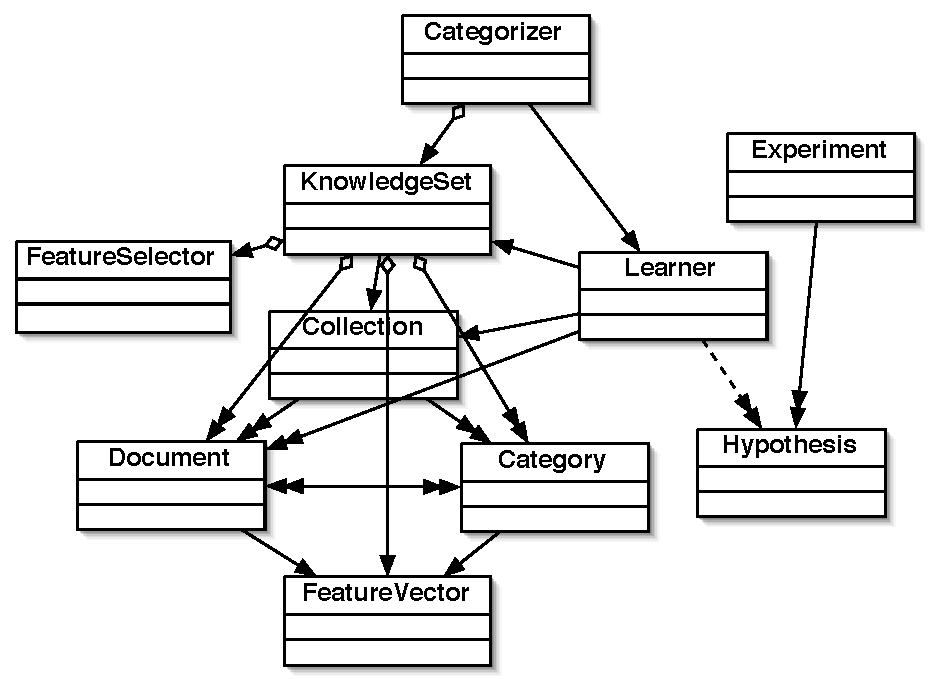
\includegraphics[width=\linewidth]{figures/classes-uml.pdf}
\caption{Class composition diagram for \aicat}
\label{classes-uml}
\end{figure}

Some examination of the basic relationships between classes and the
responsibilities of each class is helpful before looking at the design
in more detail.  The following classes form the main framework roles
in \aicat.  For exposition purposes, the UML class specification boxes
do not list every attribute and method of each class, rather only the
most important ones for this discussion.  In particular, all classes
define \method{new} constructor methods, not shown in the UML
specifications, that accept various parameters (usually corresponding
to the member attributes).  For a complete reference, please see the
\aicat\ documentation.

\section{Framework classes}
\label{framework-classes}

This section introduces each of the major \aicat\ classes as shown in
Figure \ref{classes-uml}.  For each class a partial UML class
specification rectangle is shown, indicating the attributes and
methods most important to this discussion.

\begin{concreteclass}{KnowledgeSet}
 \attributes
  \attr[Document\s]{documents} \\
  \attr{Category\s}{categories} \\
  \attr[FeatureSelector]{feature\_selector}
 \methods
  \meth{documents}{} \\
  \meth{categories}{} \\
  \meth{scan\_features}{Collection}
\end{concreteclass}

The \class{KnowledgeSet} class represents a set of processed documents, a set
of categories, and a many-to-many mapping between the two sets.
Processing may involve tokenization, stopword removal, linguistic
stemming, feature selection, and vector weighting.  Note that the term
``knowledge set'' is somewhat unique to this project, though the term
``knowledge'' is often used to describe an organization's collection
of data used as the training set $\train$ when building a TC
application.

A \class{KnowledgeSet} contains references to many \class{Document} objects and
\class{Category} objects.  It uses \class{Collection} objects to instantiate \class{Document}
and \class{Category} objects.  It uses a \class{FeatureSelector} object to perform
feature selection.  It also contains a \class{FeatureVector} object
representing the features present in all documents.


\begin{abstractclass}{FeatureSelector}
 \attributes
  \attr[number]{features\_kept}
 \methods
  \meth[FeatureVector]{reduce\_features}{FeatureVector} \\
  \meth[FeatureVector]{select\_features}{KnowledgeSet} \\
  \ameth[FeatureVector]{rank\_features}{KnowledgeSet} \\
  \ameth[FeatureVector]{scan\_features}{Collection}
\end{abstractclass}

Feature selection is performed by subclasses of the abstract \class{FeatureSelector}
class.  Each \class{KnowledgeSet} object contains a \class{FeatureSelector}
object---the \class{KnowledgeSet} provides the information necessary to do
feature selection, and the \class{FeatureSelector} performs the desired
feature selection algorithm.  A \param{features\_kept} parameter
sets an attribute of the same name in the \class{FeatureSelector}
class which controls how aggressively the features will be reduced.

The abstract \method{rank\_features} and \method{scan\_features}
methods must be implemented by concrete subclasses of
\class{FeatureSelector}.  They provide two ways to create a ranked
list of the features in a corpus.  \method{rank\_features} will
examine a \class{KnowledgeSet} object which has already been populated
with document data, returning a \class{FeatureVector} object
representing the relevance of each feature in the corpus according to
the feature selection criterion.  The \method{scan\_features} method
has the same result, but operates on a \class{Collection} object so
that the most relevant features can be determined without first having
to read the entire collection into memory.
A concrete \class{FeatureSelector::DocFrequency} subclass implements
these methods, and may therefore be used in a blackbox manner for
feature selection.


\begin{abstractclass}{Collection}
 \attributes
  \attr[hash]{category\_hash}
 \methods
  \meth[int]{count\_documents}{} \\
  \ameth[Document]{next}{} \\
  \ameth{rewind}{}
\end{abstractclass}

Because data sets in text categorization may be very large, and
because their documents may exist in several different underlying
storage mechanisms (e.g. as files in a filesystem, sections of a
larger XML file, or fields in a database), a \class{Collection} class provides
an abstract interface to a set of stored documents together with a
way to iterate through the set and return \class{Document} objects.

A concrete subclass of \class{Collection} must implement the
\method{next} and \method{re\-wind} methods for the specific kind of
iteration handled.  \method{next} should return the next document in
the collection, and \method {rewind} should reset the collection's
iterator.  This might mean re-executing a database query or moving to
the beginning of a file or directory stream.

The default implementation of \method{count\_documents} simply calls
\method{next} until all documents in the collection have been
exhausted, counting how many documents are returned.  This can
typically be replaced by a more efficient concrete implementation that
doesn't need to instantiate each document as an object.

The type of iteration to be performed, as well as the location of the
document resources, will be specified by parameters to concrete
subclasses.  Because the locations may not have any uniform structure
across subclasses (for instance, one subclass could use a path on the
local filesystem, another could use a username, password, and query
for a database, and another could use a Uniform Resource Locator for
network collections), the determination of the exact parameters to
specify is left to the subclass implementations.

A \param{category\_hash} parameter lets the caller supply a hash
relating document names to categories---if this is not provided,
category information will be determined while iterating through the
collection and processing the document data.

A \class{Collection} object may be used in several contexts within the
framework.  For instance, a \class{KnowledgeSet} instantiates its Document and
\class{Category} objects through a \class{Collection} object.  A \class{Learner} object may
also mass-categorize the \class{Documents} in a \class{Collection} object.


\begin{concreteclass}{Document}
 \attributes
  \attr[string]{name} \\
  \attr[Category\s]{categories} \\
  \attr[FeatureVector]{features}
 \methods
  \ameth{parse}{string} \\
  \meth{parse\_handle}{filehandle} \\
  \meth{create\_feature\_vector}{} \\
  \meth[FeatureVector]{features}{}
\end{concreteclass}

Each text document is represented by a \class{Document} object, or an object
of one of its subclasses.  Each document class contains methods for
turning document data into a \class{FeatureVector}.  Each document also has
a method to report which categories it belongs to.

In the standard methodology, the \method{parse} or
\method{parse\_handle} methods create plain-text data from the
native format of the document, and the
\method{create\_feature\_vector} method creates a
\class{FeatureVector} object (stored as a data member) from the text
data.  A default implementation of \method{parse} is not supplied in
the base class.

Note that the \class{Document} class is not purely an abstract class,
because a \class{Document} object may be constructed and supplied
directly with a \class{FeatureVector} object.  Perl does not enforce
the concept of abstract classes, so an unimplemented \method{parse}
method is not a problem in this case.  This can make subclassing
unnecessary for special-purpose types of ``documents'' like images or
sequences of biological data.


\begin{concreteclass}{Category}
 \attributes
  \attr[string]{name} \\
  \attr[Document\s]{documents}
 \methods
  \meth[Document\s]{documents}{} \\
  \meth[boolean]{contains\_document}{Document} \\
  \meth{FeatureVector}{features}{}
\end{concreteclass}

Each category is represented by a \class{Category} object.  Its main purpose
is to keep track of which documents belong to it, though it also
contains methods for examining statistical properties of an entire
category.

Every category must have a \param{name} string, because
\class{Collection}s will usually use the string to map between
documents and categories.  The string name is also shown to users when
presenting categorization decisions.

The \method{features} method returns a vector representing the sum of
all vectors of documents that belong to the category.  This may be
used during a Machine Learning process.  If the learner requires a
different kind of aggregate representation of a \class{Category} than
a simple vector sum, then the \method{documents} method should be used
to construct it manually.


\begin{abstractclass}{Learner}
 \attributes
 \methods
  \meth{train}{KnowledgeSet} \\
  \ameth{create\_model}{KnowledgeSet} \\
  \meth[Hypothesis]{categorize}{Document} \\
  \ameth[float]{get\_scores}{Document}
\end{abstractclass}

The abstract \class{Learner} class provides an interface to train on a
set of pre-categorized documents using the \method{train} method and
subsequently categorize previously unseen \class{Document} objects
using the \method{categorize} method.  Its
concrete subclasses implement specific categorization algorithms like
\naive\ Bayes, SVM, Decision Tree, and so on.

The \method{create\_model} and \method{get\_scores} abstract methods
need to be implemented in concrete \class{Learner} subclasses.  They
are called internally by \method{train} and \method{categorize},
respectively.  The \method{get\_scores} method returns categorization
information in terms of per-category scores and a membership
threshold.  \method{categorize} translates this data into a
\class{Hypothesis} object representing the categorization.


\begin{concreteclass}{FeatureVector}
 \attributes
  \attr[hash]{features}
 \methods
  \meth[float]{euclidean\_length}{} \\
  \meth{scale}{float} \\
  \meth[FeatureVector]{intersection}{FeatureVector} \\
  \meth[float]{dot}{FeatureVector}
\end{concreteclass}

As discussed in Section \ref{vector-space}, most categorization
algorithms don't deal directly with a document's
data, they instead deal with a \emph{vector representation} of a
document's features.  Most often, documents are represented using the
``Bag of Words'' model \cite[p. 10]{sebastiani:02}, i.e. a non-ordered, weighted set of
features.  The \class{FeatureVector} class provides an interface to the
operations one may perform on these vector representations, such as
querying features' presence or absence in a document, finding sums of
vectors, and so on.

The default implementation of the \class{FeatureVector} class stores
its data in a Perl hash.  See Section \ref{imp-featurevectors} for
discussion of an alternate approach.


\begin{concreteclass}{Hypothesis}
 \attributes
  \attr[Category\s]{all\_categories} \\
  \attr[hash]{scores} \\
  \attr[float]{threshold}
 \methods
  \meth[Category\s]{categories}{} \\
  \meth[Category]{best\_category}{} \\
  \meth[boolean]{in\_category}{Category}
\end{concreteclass}

The result of asking a \class{Learner} to categorize a previously unseen
document is a \class{Hypothesis} object.  It may be queried for information
about which categories were assigned, which category was the single
most appropriate category, what scores were assigned to each category,
and so on.

In order to support this range of behaviors, the \class{Learner} is
required to create the \class{Hypothesis} object by specifying an
appropriateness score for each category and a threshold for category
membership.  Any category whose score is above the threshold is
considered assigned by the system to the given document.


\begin{concreteclass}{Experiment}
 \attributes
  \attr[Category\s]{categories}
 \methods
  \meth{add\_hypothesis}{Hypothesis} \\
  \meth[float]{micro\_F1}{} \\
  \meth[string]{stats\_table}{}
\end{concreteclass}

The \class{Experiment} class can examine the results of many categorization
decisions (i.e., many \class{Hypothesis} objects) and may be queried for
aggregate information about the results.  This is often used in order
to determine the quality (as measured by precision, recall, error,
etc.---see Section \ref{measures}) of a \class{Learner} on a
collection of test documents.

The \class{Experiment} class uses the external module
\class{Statistics::Contingency} from CPAN to store and compute its
results.  The \class{Statistics::Contingency} module was created for
the \aicat\ project, but was split from the framework code because it
is useful for projects not involving the rest of the framework.  The
framework's \class{Experiment} class is therefore quite small,
inheriting most of its functionality from the more general-purpose
module.

\class{Experiment} contains an \method{add\_hypothesis} method for
adding \class{Hypothesis} objects to the set of data to be summarized,
and implements a \method{stats\_table} method for showing a
summary of the data in table format with a specified number of
significant figures.


\begin{concreteclass}{AI::Categorizer}
 \attributes
  \attr[KnowledgeSet]{knowledge\_set} \\
  \attr[Learner]{learner} \\
  \attr[Collection]{test\_set}
 \methods
  \meth{scan\_features}{} \\
  \meth{read\_training\_set}{} \\
  \meth{train}{} \\
  \meth{evaluate\_test\_set}{} \\
  \meth{run\_experiment}{}
\end{concreteclass}

An umbrella class \aicat\ sits above the rest of the classes
providing a convenient interface to a complete system for text
categorization.  Most applications built using the framework will
instantiate an object of this class.  Note that the term \aicat\ can
refer either to the framework as a whole, or to the umbrella class.
The distinction will be made clear in this text where it is necessary
to do so.

The main benefits of having an umbrella class in the framework are
that the object constructor mechanism described in Section
\ref{factory-method} can operate consistently across the entire
framework, and that it provides a very high-level interface, requiring
very little application-specific code to invoke the framework's
functionality.

The most important attributes of the \aicat\ class are a
\class{Learner}, a \class{KnowledgeSet} that the \class{Learner}
trains on, and a \class{Collection} of documents that the
\class{Learner} can be tested on.  Because not every usage of this
class need involve both training and testing, the \class{KnowledgeSet}
and \class{Collection} attributes may be null if they are not needed
by the particular application.

The \method{scan\_features} method invokes feature selection using the
\class{KnowledgeSet}'s \class{FeatureSelector}.  The resultant list of
desired features can be used by the \method{read\_training\_set}
method which populates the \class{KnowledgeSet} with data from the
training corpus.  The \method{train} method invokes the
\class{Learner}'s \method{train} method on the \class{KnowledgeSet},
and the \method{evaluate\_test\_set} method invokes the
\class{Learner}'s \method{categorize\_collection} method on the test
collection.  A \method{run\_experiment} method automates the running
of these four methods and shows the user a summary of the results.


\section{Design Patterns in \aicat}

The real power and intellectual content of any framework lies not in
the design of its individual classes, but in the interfaces between
the classes and the way objects collaborate to solve problems in the
framework's application domain \cite[p. 31]{fayad:99}. These
relationships can be quite complicated and difficult to explain, yet
understanding them is essential to understanding the framework.

In this section, certain important local structures in the \aicat\
framework design will be discussed using the language of design
patterns (see Section \ref{patterns}).  The ``Iterator,'' ``Composite,'' ``Adapter,'' ``Strategy,''
and ``Factory Method'' patterns are discussed, and specific examples
from \aicat\ show how they are applied within the framework.  These
are not by any means the only instances of common design patterns in
the framework, nor do the specific patterns in \cite{gamma:95} provide
a complete catalog of all possible patterns in software.  This
discussion also does not give complete coverage to all design-related
issues involved in \aicat.  But patterns often provide a starting
point for design discussion, and their use has been found beneficial
in many diverse arenas \cite{granlund:99}, so they are used here in
the hope that they clarify the important design issues.

\subsection{Iterator}

The Iterator pattern provides ``a way to access the elements of an
aggregate object sequentially without exposing its underlying
representation.'' \cite[p. 257]{gamma:95} Its main purpose is to
decouple the traversal process on an object's aggregate members from
the object's internal data structure implementation.  In this way,
clients can iterate through aggregate objects without knowing the
objects' internal structure.

In the \aicat\ framework, it is often necessary to iterate
through collections of documents and perform some action on them.  For
example, the documents may form a training set for a \class{Learner} to base a
model on, or they may form a test set on which to evaluate the model.

The \class{Collection} class implements the Iterator pattern
\cite[p. 257]{gamma:95} over documents in the framework.  Figure
\ref{Iterator-collection} shows the main relationships involved in
this pattern.

\begin{figure}
\includegraphics[width=\linewidth]{figures/Iterator.pdf}
\caption{The Iterator pattern in the \class{Collection} class}
\label{Iterator-collection}
\end{figure}


\cite[p. 259]{gamma:95} suggests that the most common reasons for
using a formal custom iterator are:

\begin{itemize}

\item to access an aggregate object's contents without exposing its
internal representation.

\item to support multiple traversals of aggregate objects.

\item to provide a uniform interface for traversing different
aggregate structures.

\end{itemize}

The first and third reasons are most germane to the TC document iteration
process.  As explained in section \ref{Document storage}, it is
important that the framework can directly import documents from their
various underlying storage mechanisms in order to prevent unnecessary
duplication of data.  In order to hide the details of the storage
mechanism from the rest of the framework, a \class{Collection} object
retrieves documents from the storage mechanism and returns them
as \class{Document} objects.  It provides a unified interface to iteration
over stored documents so that the various classes that need to perform
this iteration (chiefly \class{Learner} and \class{KnowledgeSet}) don't need to be
aware of storage issues.  In this sense, the ``internal
representation'' of the aggregate structure is often external to the
framework itself---it may be files in a filesystem, entries in a
database, records in an XML document, or another mechanism.

In addition to providing a generic interface to a stored collection of
documents, the Iterator pattern allows clients of the \class{Collection} class
to use memory efficiently.  A \class{Collection} object will typically defer
creation of its \class{Document} objects until its client calls its
\method{next} method.  In this way, the \class{Collection} doesn't store all
the \class{Document} objects in memory simultaneously---if the client needs to do so,
it can, or it can merely query properties of each document and dispose
of them in turn.

Note that the \class{Collection} class defines a \method{next} method,
but no \method{previous} method.  This is largely because common
document storage mechanisms like filesystems or databases typically
only have one-directional iterators.  Insisting that
\class{Collection} classes needed to implement a \method{previous}
method to support bidirectional iteration would impose an
unreasonable burden on them.

In order to decouple the storage mechanism from the internal format of
documents (see section \ref{Document format}), \class{Collection}
classes can cooperate with any subclass of the \class{Document} class.
The client of the \class{Collection} class informs it that it should
instantiate documents using a certain \class{Document} subclass.
Since the \class{Document} subclasses share a common interface, \class{Collection}
may remain ignorant of all internal document formatting issues,
passing data to the proper constructors in order to instantiate
\class{Document} objects.


\subsection{Composite}

The Composite pattern ``lets clients treat individual objects and
compositions of objects uniformly.'' \cite[p. 163]{gamma:95} It is
often used to represent trees or other data structures in which the
form of a subset of the structure is not qualitatively different from
the form of the entire structure.  In simple terms, this means that
the same kinds of operations---iteration over sub-nodes, inspection of
the root node, and so on---can be performed on the entire tree, a
subtree, or even a single node.

In fact, the Composite pattern does not apply only to tree
structures.  It applies whenever a self-similarity exists between the
whole and the parts in a part-whole hierarchy.

One instance of this kind of structure in Text Categorization is in
so-called ``ensemble learners,'' also known as ``classifier
committees.''  An ensemble learner is a categorizer that combines the
results of a set of other categorizers in some way to arrive at a
categorization result of its own \cite[p. 30]{sebastiani:02}. Often,
an ensemble learner may outperform each of its constituent members on
the general categorization task  \cite{tumer:98}.

To implement ensemble learners within \aicat, the Composite
pattern may be applied to the \class{Learner} class to create a
\class{Learner::Ensemble} subclass.  Figure \ref{Composite-ensemble}
shows the classes participating in this pattern.

\begin{figure}
\includegraphics[width=\linewidth]{figures/Composite.pdf}
\caption{The Composite pattern in the \class{Learner::Ensemble} class}
\label{Composite-ensemble}
\end{figure}

Since \class{Learner::Ensemble} is a subclass of the abstract
\class{Learner} class, it conforms to the \class{Learner} interface.
This is crucial to implementation of the Composite pattern---it means
that clients may use the \class{Learner::Ensemble} class without
knowing that it implements an ensemble learner behind the scenes.  In
this way, transparent ensemble learning is achieved through
polymorphism.

According to \cite[p. 30]{sebastiani:02}, ensemble learning techniques
can be specified by (1) a set of individual learners (the ``members''
in Figure \ref{Composite-ensemble}), and (2) a mechanism for combining
the output of the individual learners.  The \class{Learner::Ensemble}
class can provide generic support for creating the member learners of
the ensemble, but the combination mechanism may take many different
forms.  Such algorithms are an active area of Machine Learning
research.  As such, \class{Learner::Ensemble} may be subclassed in
order to implement different combination mechanisms.  Since these
subclasses implement the combination algorithm in different ways, they
may themselves be seen as carrying out a Strategy pattern (see section
\ref{Strategy}).


\subsection{Adapter}

The Adapter pattern ``converts the interface of a class into another
interface clients expect.'' \cite[p. 139]{gamma:95} It is commonly
used when an existing resource provides the functionality necessary
for a certain task, but the interface of that resource doesn't match
the interface necessary for the environment in which that task must be
performed.  For example, a framework may require that a particular
role is implemented by subclasses of a certain abstract class.  This
helps unify functionality by taking advantage of polymorphic
abstraction \cite[p. 5]{fayad:99}. That functionality may already be
present in an existing body of code outside the framework.  An Adapter
can help bridge the gap between the two code bodies by letting the
external code function inside the framework.\footnote{An Adapter may
sometimes be called a Wrapper.  Both terms will be used in this
discussion.}

Many developers in the text categorization community create their
software as demonstrations of novel algorithms, or as stand-alone
libraries that implement one small part of the overall text
categorization task.  The majority of cutting-edge research will be
implemented in this way, if a public implementation is available at
all.  In order to leverage this work for a categorization framework,
some adaptation is invariably necessary.  Unless a developer happened
to be using \aicat\ as a development environment, her implementation
will not be directly usable as a framework element.  Thus Adapters
provide a mechanism for keeping the framework current with advances in
the field of text categorization.

\begin{figure}
\includegraphics[width=\linewidth]{figures/Adapter.pdf}
\caption{The Adapter pattern in the Learner class}
\label{Adapter-learner}
\end{figure}

Figure \ref{Adapter-learner} shows how the Adapter
pattern is present in \aicat's \class{Learner} class.  The abstract
\class{Learner} class specifies a common interface that all subclasses
must conform to.  Several of its concrete subclasses implement their
functionality using a framework-external resource.  For example,
\class{Learner::DecisionTree} uses the stand-alone module
\class{AI::DecisionTree} for implementation.  \class{Learner::Weka}
is a wrapper around the ``Weka'' Machine Learning system.
\class{Learner::SVM} is a wrapper around a framework-external
\class{Algorithm::SVM} module, which is itself a wrapper around the
\texttt{libsvm}\cite{libsvm} C library.\footnote{Note that
\class{Learner::SVM}, Weka, and \texttt{libsvm} are not part of the
contributed work of this thesis, as they are written by other authors.}

Note that these four Adapter examples exhibit three very different
applications of the Adapter pattern.  \class{Learner::DecisionTree}
exhibits a very straightforward Adapter usage as presented in
\cite{gamma:95}---an existing stand-alone class exists that implements the
needed functionality, and its interface is adapted to the framework
requirements by a simple wrapping subclass.  The \class{Learner::SVM}
wrapper is also fairly straightforward.  The other two wrappers,
however, reflect the highly heterogeneous nature of the text
categorization domain.  The main reason for the adaptation in the
\class{Algorithm::SVM} class is to provide a Perl interface to a C
library.  The \class{Learner::Weka} adapter combines language
adaptation (in this case, Java to Perl) with functionality
transformation (mapping Weka's methods to the required \class{Learner}
interface).

Adapters can create design flexibility.
The current implementation of \class{Learner::Weka} interfaces with
Weka through its command-line interface, but this is not a design
constraint.  Future implementations may embed the Weka system inside
the \class{Learner::Weka} module for reasons of efficiency or platform
compatibility.  Because this interface is hidden using an Adapter
pattern, the implementation may be changed freely.

The differences in interfaces between the Adapter and the Adaptee may
be merely historical, or they may reflect different needs in different
domains.  The Adapter must conform to the interface of its abstract
superclass, which is typically designed to be independent of subclass
abilities and implementations.  The Adaptee may be designed for use in
a different arena, with extra functionality or an interface that
takes full advantage of its capabilities.

Using Adapters may bring major benefits in the area of reusability.
Obviously, classes won't have to be re-implemented if the
functionality can be adapted from an existing implementation.  Second,
and perhaps more importantly, classes initially implemented for a
framework may be converted into Adaptee classes that are usable in isolation.
This can bring them better exposure in other projects and thus more
feedback, maturing them quickly.  This can be a major win, because
iteration is considered a limiting factor in framework development
\cite[p. 75]{fayad:99}, so any process that speeds up maturity in
framework components can have a large impact.  Adapters can also force
a more robust encapsulation of design in the Adaptee, bringing
benefits in the conceptual and technical segmentation of the
framework.

\subsection{Strategy}
\label{Strategy}

The Strategy pattern defines ``a family of algorithms, encapsulates
each one, and makes them interchangeable'' \cite[p. 315]{gamma:95}.
It is used when a domain task needs to be carried out, but there may
be several ways to carry out that task, and it is important to let the
user or client choose from among these alternatives.

An important concept in the Strategy pattern is that of ``behavior.''
In \cite{gamma:95}, the Strategy pattern is recommended when ``many
related classes differ only in their behavior.''  In this context, a
distinction is made between an algorithm's purpose and its behavior.
For example, a set of algorithms for finding line-break points in text
paragraphs have a common purpose (to accomplish the line-breaking
task), but they may carry out their task in different ways.  The
algorithms may make different trade-offs in terms of speed and memory,
or they may try to optimize different aspects of the task.  Since it
is impossible to satisfy all clients in all situations with a single
choice of algorithm, it is desirable to encapsulate each algorithm in
a class that can be chosen or extended by the client.

The field of text categorization has several natural applications for
the Strategy pattern.  One of the primary concerns of most TC
researchers is the development of novel algorithms for various aspects
of the categorization task, so it is essential for these algorithms to
be easy to vary in a categorization framework.  In the language of
\cite{fayad:99}, these algorithms are framework ``hot spots.''

The most obvious Strategy application in \aicat\ is the
\class{Learner} class and its subclasses.  These classes all have a
common task to perform: that of training a categorizer and
categorizing unseen documents.  The various subclasses represent very
different ways to accomplish that task.  Importantly, the results of
the task, and not just the internal mechanism that performs it, may be
different depending on which \class{Learner} subclass is used.

\begin{figure}
\includegraphics[width=\linewidth]{figures/Strategy.pdf}
\caption{The Strategy pattern in the Learner class}
\label{Strategy-learner}
\end{figure}

Figure \ref{Strategy-learner} shows how the Strategy pattern appears
in the \class{Learner} class and its subclasses.  Three concrete
subclasses are shown that implement specific Machine Learning
algorithms (see Figure \ref{inheritance-uml} for other \class{Learner}
subclasses currently implemented).  From the point of view of the
client \aicat\ object, all \class{Learner}s have the same interface
and may therefore be treated uniformly.  The framework user or
application designer, however, may choose judiciously among subclasses
depending on the particular needs of the application.  Customizability
of the Machine Learning algorithm is of paramount importance to the
framework since it would be useless to most researchers if this were
not the case.  Many researchers may wish to write their own
\class{Learner} subclasses using this portion of the framework in the
``whitebox'' paradigm.  Other researchers, and most application
developers, will want to use existing framework classes in a
``blackbox'' framework usage style \cite[p. 10]{fayad:99}.  Either
method is supported.

Each \class{Learner} subclass must implement the abstract
\method{train} and \method{categorize} methods in order to perform the
two essential tasks of any \class{Learner}.  The \method{train} method
examines a \class{KnowledgeSet} object and builds an internal (and
opaque) model that will be used to categorize future documents.  The
\method{categorize} method takes a \class{Document} object as an
argument and returns a \class{Hypothesis} object representing the
outcome of categorization based on the model.

\begin{figure}
\includegraphics[width=\linewidth]{figures/Strategy-feasel.pdf}
\caption{The Strategy pattern in the FeatureSelector class}
\label{Strategy-feasel}
\end{figure}

Another application of the Strategy pattern is shown in Figure
\ref{Strategy-feasel}.  Here, the varying algorithm performs
feature selection, another framework hot spot.  There has been much
activity in current research on improving feature selection for
different scenarios \cite{yang:01,yang:97}, so customization in this
area is also essential.

To perform feature selection, a \class{KnowledgeSet} object invokes
either the \method{select\_features} or \method{scan\_features} method
of the \class{FeatureSelector} object, depending on whether a complete
\class{KnowledgeSet} or a \class{Collection} object should be
examined.  Examining a \class{Collection} iteratively requires less
memory because the documents don't have to be loaded into memory all
at once, but it requires a separate pass through the data.  The choice
of which method to run is made in response to user specification.

Because \method{select\_features} and \method{scan\_features} are
virtual methods in the parent class, any concrete subclass must
implement these methods according to the particular algorithm the
subclass represents.  As of this writing, only the
\class{FeatureSelector::DocFrequency} subclass is implemented, but
the other subclasses in the diagram are planned.


\subsection{Factory Method}
\label{factory-method}

In any framework of sufficient size and customizability, attention
must be paid to the issue of how specific classes are chosen for the
various framework roles, how these classes are instantiated, and how
the instantiated objects are connected to each other.  In the simplest
possible case for the framework developer, the framework client code must create all objects and
manually connect them to each other.  For instance, in \aicat, the
client code might create a \class{KnowledgeSet} object, a
\class{Learner} object, an \aicat\ object, a \class{Collection}
object, then populate the \aicat\ object with \class{KnowledgeSet} and
\class{Learner} objects, and the \class{KnowledgeSet} with a
\class{Collection}, thus satisfying the structural relationships
indicated in Figure \ref{classes-uml} on page \pageref{classes-uml}.
An approach like this is diagrammed in Figure
\ref{naive-constructors}.

\begin{figure}
\includegraphics[width=\linewidth]{figures/naive-constructors.pdf}
\caption{A client-side approach to object construction}
\label{naive-constructors}
\end{figure}

This approach works, but it is error-prone and cumbersome.  It forces
every client to specify the framework relationships explicitly, when
in fact these are fundamental relationships of the \emph{framework},
not of the client code.  It makes little sense for this structural
code to be outside the framework and even less sense for it to be
duplicated in every application that uses the framework.  Note too
that Figure \ref{naive-constructors} only shows a small part of the
framework being used---in reality, the client code would have to
accept responsibility for creating all the objects in the framework,
not just the four pictured here.

For these reasons, it is often better if the framework can provide
support for object creation and enforcement of the framework
relationships.  An example of this situation is pictured in Figure
\ref{better-constructors}.  Here, the patterns of object creation more
closely follow the class relationships that will be used at runtime.
This design is moving closer toward a factory-style pattern in which
object creation is delegated to another object \cite{gamma:95}.
defines two specific kinds of factory patterns: ``Factory Methods''
and ``Abstract Factories.''  Figure \ref{better-constructors} does not
fit either of these patterns exactly, but it does fall under the
general category of factory object creation.

\begin{figure}
\includegraphics[width=\linewidth]{figures/better-constructors.pdf}
\caption{A framework-side approach to object construction}
\label{better-constructors}
\end{figure}

A scheme like that in Figure \ref{better-constructors} has both
advantages and disadvantages compared with that in Figure
\ref{naive-constructors}.  One obvious advantage is that the client
code is greatly simplified, because it needn't create any framework
objects except the top-level object, and because it doesn't have to
link the objects to each other.  This eliminates redundancy in
multiple client code bases and allows the framework designer greater
flexibility in redesigning the framework hierarchy.  Another advantage
is that the framework objects are created by the objects that use
them, so class code can accept responsibility for its subordinate
objects' entire life cycles.

However, these properties can also be seen as disadvantages.  If each
framework object assumes all responsibility for creating its
subordinate objects, then the client may not be able to control the
creation process effectively.  This is a problem for at least two
important reasons.  First, the client may wish to change some
properties of the objects it creates.  If it passes all constructor
parameters to the top-level class constructor, then this constructor
must have knowledge of all of its subordinate classes' parameters in
order to affect their construction correctly.  This would couple the
framework classes too closely.  Second, the client may (and frequently
will) change which classes are participating in the framework
hierarchy.  If the \class{KnowledgeSet} class always creates a certain
class of \class{Collection} object, then in order to substitute a
different \class{Collection} class, the \class{KnowledgeSet} class
would need to be subclassed---this means the top-level \aicat\ class would
also need to be subclassed in order to create the new type of
\class{KnowledgeSet}, leading to a proliferation of subclasses just to
manage object creation.  Clearly a better solution is needed.

In order to create a proper solution, some analysis of the problem is
warranted.  Part of the reason these creational issues are difficult
is that no standard method exists to translate the framework's design
relationships into code.  Common programming languages have no
built-in support for managing the patterns of creation necessary in
frameworks.  Contrast this with inheritance relationships, which are
directly supported by object-oriented languages.  For instance, a C++
or Java \texttt{class} declaration lists its superclasses explicitly,
and Perl specifies inheritance via each class's \texttt{@ISA} array.
Because inheritance is directly implemented by the language, it is
easy for framework users to understand inheritance relationships, and
these relationships are expressed straightforwardly in the framework
code.  For support of this point, consider object-oriented programming
in languages like C that don't have inherent OO support.
Understanding the inheritance structures can be much more
challenging in this situation \cite[p. 7]{fayad:99}.

With this perspective in mind, one solution is to create a way for
each class to explicitly declare its constructor parameters and its
relationships to other classes, and then let the framework manage
object creation in a consistent, centralized manner based on these
declarations.  In a sense, this approach extends the implementation
language to be able to express the important framework relationships
directly rather than letting them emerge implicitly from patterns of
usage in the code.  Client code then supplies parameters that inform
the top-level object about which classes should be instantiated and
what parameters should be passed to each class's constructors, and the
framework itself directs the object creation process.

\begin{figure}
\includegraphics[width=\linewidth]{figures/factory-constructors.pdf}
\caption{A centralized approach to object construction}
\label{factory-constructors}
\end{figure}

Because many users of an application framework will be hesitant to
depend on a modified, nonstandard version of the implementation
language, \aicat\ uses inheritance to add these explicit declaration
capabilities to every class participating in the framework hierarchy.
Figure \ref{factory-constructors} shows an example of how this
inheritance functions.  The abstract \aclass{ObjectFactory}
class\footnote{The \aclass{ObjectFactory} name is used here only for
discussion purposes.  See Section \ref{constructor-methods} for the actual
implementation details.} adds the ability for any class derived from
it to declare the relationships discussed in the previous paragraph.
It also manages the creation of subordinate objects.  For instance,
the top-level \aicat\ class declares that it contains both a
\class{KnowledgeSet} and \class{Learner} object in an aggregation
relationship.  When an \aicat\ object is created, \class{KnowledgeSet}
and \class{Learner} objects will automatically be created by the
\aclass{ObjectFactory} according to the client code's parameters.  The
\class{KnowledgeSet} also declares that it will need to create
\class{Collection} objects on demand, and calls creational methods
provided by its \aclass{ObjectFactory} superclass when it needs to
create them.

It is important to note that this is not a direct application of
either the Factory Method or Abstract Factory patterns in
\cite{gamma:95}.  The standard Factory Method pattern requires
separate subclasses to create the concrete subclasses.  A closer
variation is the ``Parameterized Factory Method''
\cite[p. 110]{gamma:95}, which lets the specific subordinate class
be determined by switching among several known classes.  This is
closer to the data-driven approach employed in \aicat, but it doesn't
address the issue of how the subordinate classes must actually be
created at runtime.  The Abstract Factory pattern is also similar in
that the creation of multiple objects is centralized, but in \aicat\ a
separate factory object is not necessary.

This approach effectively solves the problems with the first two
approaches considered here.  The client code is freed from having to
create multiple framework objects, and the framework relationships are
expressed explicitly in the framework code, not in the client code or
implicitly in the framework implementation.  Clients are also able to
easily change which classes participate in the framework hierarchy
and can specify constructor parameters without invoking the
constructors directly.  Framework code doesn't create subordinate
objects directly, but defers creation to factory methods inherited
from superclasses.  In this way, subclassing is kept to a minimum, and
the framework runtime structure can be highly parameterized.

\section{Examples}

Effective documentation is essential for the use and dissemination of
any framework \cite[ch. 21]{fayad:99}. The \aicat\ distribution
contains complete documentation of the user-visible classes.  That
documentation will not be reproduced here.  Of use to the present
discussion, however, are some simple examples of using the framework.
Example code often forms one of the most important kinds of framework
documentation since it shows concrete examples of framework
usage \cite[p. 498]{fayad:99}.

Figure \ref{high-level-interface} shows the highest-level
interface usage, in which an entire experi\-ment---training on a
training corpus, testing on a test set, and showing results to
the user---is performed by setting appropriate parameters in
the constructor of the highest-level \aicat\ object.  These parameters
may include \param{learner\_class} for specifying the class of machine
learner that should be used, \param{stopword\_file} for specifying a
file containing a list of stop words, or \param{stemming} to indicate
what type of linguistic stemming, if any, should be performed on the
document data.  The generic Factory Method mechanism described in
Section \ref{factory-method} ensures that each parameter becomes an
argument to the appropriate object constructor method.

\begin{figure}
\begin{code}
use AI::Categorizer;
my $c = new AI::Categorizer(...parameters...);
$c->run_experiment;
\end{code}
\caption{Highest-level interface to \aicat}
\label{high-level-interface}
\end{figure}

Figure \ref{medium-level-interface} shows a slightly lower-level
interface to the framework.  Here, the individual stages of the
\method{run\_experiment} method from Figure \ref{high-level-interface}
are run separately, and may in fact be run in separate programs on
different machines if the \param{progress\_file} parameter is used in
order to save state between the stages.

\begin{figure}
\begin{code}
use AI::Categorizer;
my $c = new AI::Categorizer(...parameters...);

# Run the separate parts of $c->run_experiment
$c->scan_features;
$c->read_training_set;
$c->train;
$c->evaluate_test_set;
print $c->stats_table;
\end{code}
\caption{Separate invocations of experimental phases}
\label{medium-level-interface}
\end{figure}

In an applied setting, the application developer may need much finer
control over the object behavior.  For instance, the developer may not
be very interested in the overall performance on a test set, but
rather in the specific decisions of the trained categorizer on
documents presented to it by users.  Figure
\ref{application-interface} demonstrates one simple such application,
in which the trained categorizer is loaded into memory using the
\method{restore\_state} method (see Section \ref{saving-state}), then repeatedly asked to categorize
documents using the \method{categorize} method.  Here the application
uses the \method{best\_category} method to select only the single
category with the best score, but another application may require
different information from the \class{Hypothesis} object \texttt{\$h}.

\begin{figure}
\begin{code}
my $l = AI::Categorizer::Learner->restore_state(...);
while (...) {
  my $d = ...create a document...
  my $h = $l->categorize($d);
  print "Best category: ", $h->best_category, "\n";
}
\end{code}
\caption{Using \aicat\ for direct categorization of documents}
\label{application-interface}
\end{figure}



\section{Limitations}

In any software design process, choices must be made that determine
the scope and direction of the project.  In designing \aicat, these
choices have been made in a way that tries to maximize the usefulness for
the intended audience, the reuse of framework components, the framework's
efficiency and flexibility, and the rapid development of applications.  In
some cases, these decisions may limit the capabilities of the
framework.  This section describes some of these limitations, explains
the reasons for them, and proposes alternative ways to deal with the
problems they present.

\subsection{Structured Feature Vectors}

The basic data model representing documents in the \aicat\ framework
is the feature vector.  In this model, certain features of each
document (typically counts of words or word stems) are measured, and
their values are represented as vectors in a vector space encompassing
all document vectors in the training set.  Each document vector is
\emph{flat}, i.e. an $n$-dimensional vector with no internal
structure, where $n$ is the total number of features in all the
training documents.  This representation has been shown to be very
effective for Text Categorization applications
\cite[p. 10]{sebastiani:02} and is crucial for such common TC
algorithms as k-Nearest-Neighbor and Support Vector Machines.

However, many environments routinely use richer data models for
documents.  For instance, researchers in the Linguistics community
often represent documents as hierarchical data structures indicating
each syntactical element's relationship to the other syntactical
elements in the document \cite[ch. 11 \& 12]{manning:99} \cite{sag:99}.
Additionally, many structured HTML and XML business documents are
represented using the Document Object Model, which provides a common
programmatic interface to the logical structure of
documents \cite{dom}.

Because few TC techniques in the common literature take advantage of
document structure, and because several techniques depend on
unstructured vector representations, the \class{FeatureVector} class
only provides an interface to unstructured feature vectors.  This
class does leave the \emph{implementation} of the vectors unspecified,
however, so that different internal representations are possible (see
Section \ref{imp-featurevectors} for more on this topic).

In an application using structured documents, two options exist for
taking advantage of this structure using \aicat.  One option is to
``flatten'' the structure of the document into a traditional feature
vector representation.  Unfortunately, it is not always clear to the
developer how this flattening should be done, and the flattening
process may lose valuable information about document structure, making
categorization results sub-optimal.

Another option if the document structure is just a sequence of
document sections and not arbitrarily nested structures is to use the
\aicat\ framework's \param{content\_weights} parameter.  This allows
each document to be divided into an arbitrary number of sections such
as title, abstract, body, and so on, assigning ``importance'' weights
to each section.  These weights will be used when creating a feature
vector from the document content, in effect automatically flattening
the document into a traditional feature vector.

Neither of these two solutions allow the framework to truly deal with
arbitrarily structured documents in any natural way.  It is therefore
to be understood that the framework is not currently capable of
exploiting this structure very deeply, and this is a possible area of
future work.

\subsection{Hierarchical Categorization}
\label{hierarchical}

Hierarchical categorization is the process of categorizing documents
into a set of categories possessing a treelike structure.  The
hierarchical nature of the category set may be exploited for both
increased efficiency and improved accuracy \cite{dumais:00}.  Because
some common categorization problems are inherently hierarchical, the
field of hierarchical categorization has seen significant attention in
the research literature \cite[p. 7]{sebastiani:02}.

In the \aicat\ framework, hierarchical categorization has not
explicitly been supported in the architecture.  The set of categories
in any framework categorization task is assumed to be a simple list of
named sets of documents with no hierarchical structure.  However,
there are at least two ways of dealing with hierarchical
categorization tasks using the framework.

The first way is to simply transform the hierarchical set of
categories into a simple flat list, by prepending each category's name
with the names of all its parent categories.  In this way, the
framework will assign any category in the flat list of categories, and
then the results can be transformed back into members of the
hierarchical category set.  The main advantage of this technique is
that it is simple to apply, with a natural and transparent
transformation between structured and flat category sets.  The main
disadvantage is that the system is not really performing hierarchical
categorization at all, so it is not taking advantage of any of the
hierarchical category structure for efficiency or accuracy
improvements.

The second way to achieve hierarchical categorization using \aicat\ is
to manually break the categorization task into several smaller tasks,
building a separate machine learner for each splitting node in the
category hierarchy.  This is a common approach to hierarchical
categorization in the literature
\cite{dumais:00,koller:97,chakrabarti:98}, and it seems to naturally map
the hierarchical problem into a hierarchical solution.  The main
disadvantage with this method is that the framework provides no direct
support for creating a hierarchy of categorizers, so the client
must create and maintain code for the
hierarchical aspect of the task.  This is another possible area of
future work, and a fellow student in the Web Engineering Group at
Sydney University is currently working toward a solution for using
\aicat\ in hierarchical categorization.

\chapter{Implementation}
\label{Implementation}

With the functionality requirements and class designs in Chapter
\ref{design} as a guide, the \aicat\ framework has been implemented
and released under an open source license\cite{raymond:97,dibona:99} as a
part of this thesis and as a continuing project in Text
Categorization.  This chapter describes some of the implementation
decisions that have been made in \aicat\, and provides some of the
reasoning behind them.

\section{Implementation Language}

In order to provide maximum support for the kinds of real-world
scenarios described in Section \ref{use-cases}, it was determined that
a broad-coverage, widely-used programming language should be used to
implement the \aicat\ framework.  Three extremely common
object-oriented languages fulfilling these criteria are \texttt{C} (or
rather its object-oriented derivatives like \texttt{C++} and
Objective-\texttt{C}), Java, and Perl.  Each of these languages has
its advantages and disadvantages, and a full comparison between them
is beyond the scope of this thesis.  Perl was ultimately chosen for
the \aicat\ project, which provides the following benefits.

\begin{itemize}
\item Perl is widely known to be a powerful text processing tool
   \cite{friedl:02, pedersen:01} \cite[p. 121]{manning:99}, hence it should be
   relatively easy for users of the framework to customize its
   processing capabilities.
\item A large number of contributed Perl modules are freely available
   for many different tasks on the CPAN \cite{cpan}, which extends the
   domain of applicability of the framework.
\item Perl is an expressive high-level language that allows for rapid
   prototyping, so the framework developers and application developers
   can experiment with several alternative designs fairly quickly.
\item Perl is widely deployed and is part of all standard Unix
   distributions.  It is available for most platforms that have a
   \texttt{C} compiler, and because of common high-level interfaces,
   Perl code written on one platform is often more portable to other
   platforms than the equivalent \texttt{C} code would be.
\item Perl can be embedded within applications written in other
   languages, particularly in \texttt{C}/\texttt{C++} applications
   using Perl's embedding interface, or in Java applications using the
   JPL toolkit.  This allows for maximum reusability of the
   framework as described in Section \ref{embedded-apps}.
\item Code from other languages can be embedded within Perl
   applications, using either the XS extension mechanism for
   \texttt{C} code, or the Inline embedding mechanism for several
   languages, including \texttt{C} and its derivatives, Java, Tcl,
   Assembler, and Python, among others.  This allows the framework to
   use efficient data structures and algorithms implemented in other
   languages if necessary, while keeping the convenient high-level
   interface in Perl.  It also allows integration with existing code
   libraries from various sources without locking the developer into a
   language choice.
\item There is an active community of users interested in using a
   Perl-native text categorization framework.  This community can
   contribute back to the framework project.  Several community
   members have already contributed feedback, bug fixes, and
   application ideas for the \aicat\ project.
\end{itemize}

\section{Framework constructor methods}
\label{constructor-methods}

To implement the behavior discussed in Sections \ref{ml-config} and \ref{factory-method},
the \class{Class::Con\-tain\-er} module from CPAN\footnote{The
\class{Class::Container} module was written by Ken Williams for a
previous project\cite{rolsky:02} and greatly extended for the \aicat\
project.} implements the abstract parent class \aclass{ObjectFactory}
shown in Figure \ref{factory-constructors}.  It provides the generic
specification of object constructor parameters, as well as generic
mechanisms for creating subordinate objects within the framework.

\begin{figure}
\begin{verbatim}

package AI::Categorizer::Learner;
use base 'Class::Container';
use Params::Validate qw(:types);

__PACKAGE__->valid_params
  (
   knowledge_set  => { isa => 'AI::Categorizer::KnowledgeSet',
                       optional => 1 },
   verbose        => { type => SCALAR,
                       default => 0 },
  );

__PACKAGE__->contained_objects
  (
   hypothesis => { class => 'AI::Categorizer::Hypothesis',
                   delayed => 1 },
   experiment => { class => 'AI::Categorizer::Experiment',
                   delayed => 1 },
  );

\end{verbatim}
\caption{An example of \class{Class::Container} usage from the \class{Learner} class}
\label{class-container}
\end{figure}

Figure \ref{class-container} shows a simplified example of
\class{Class::Container} usage in the \class{Learner} class from \aicat.  The
\method{valid\_params} and \method{contained\_objects} class methods are
inherited from the superclass \class{Class::Container}, and they
provide the mechanism by which each class can declare its main
constructor interface.  In this case, the \class{Learner} class
declares that it accepts two constructor parameters, called
\param{knowledge\_set} (a \class{KnowledgeSet} object which will form
the training set for the learner) and \param{verbose} (an integer
specifying the amount of status information to show the user during
the training process).

The \method{contained\_objects} method lets the \class{Learner} class
declare its subordinate objects in the framework architecture.  In
this case, each \class{Learner} will create \class{Hypothesis} and
\class{Experiment} objects at runtime; \class{Hypothesis} objects are
created in the \method{categorize} method when any document is
categorized, and \class{Experiment} objects are created in the
\method{categorize\_collection} method to organize and report the
results of categorizing many documents.  The \class{Learner} will
create these objects on demand using \method{create\_delayed\_object},
also inherited from \class{Class::Container}, as a factory method.  In
the object specification, the ``delayed'' flag indicates that the
objects will be created on demand in this manner---if this flag were
not specified, the objects would be automatically created during the
\method{new} method in an aggregation\cite[p. 22]{gamma:95}
manner.


\section{Data Structures}

To a large extent, the data structures used in \aicat\ are
unspecified, since the framework specification dictates only the
framework interface methods and the relationships among classes.
However, the concrete implementations of several classes must choose
implementation details, and those details are described here.

\subsection{Feature Vectors}
\label{imp-featurevectors}

Many parts of the framework code must manipulate feature vectors,
which we define as a set of key-value pairs relating document features
(which may be words, word stems, 2-word combinations [bigrams], or
other derivatives of document data) to values (which may be frequency
counts or other weighted measures of importance).  Some examples of
this include the features of an individual document, the aggregated
features of a knowledge set or of the documents belonging to a
particular category, or a vector of features whose weights have been
assigned by a particular \class{Learner} implementation.

The \class{FeatureVector} class provides both a concrete
implementation of a feature vector interface, and a base class from
which other classes may inherit if they wish to use a different
internal representation of the data or extend the capabilities of the
base class.  Perl provides hash tables (sometimes called
``dictionaries'' in some languages) as a language-level data
structure, and the default implementation in \class{FeatureVector}
uses these as its mapping between features and values.  This provides
the following benefits:

\begin{itemize}
\item Insertions, deletions, and lookups are all $O[1]$
  operations, so the size of the feature set can grow without any
  penalty on the time to perform these operations.
\item Hashes can store \emph{sparse} information efficiently, meaning
  that only nonzero entries in a vector need to be stored.  This can
  be important if the dimensionality of the ambient vector space is
  very large, because memory savings of 1-3 orders of magnitude may be
  realized.
\item The hash data structure stores the key as a string.  This may be
  the word or word stem from the document itself, avoiding the need to
  use a separate lookup table to translate from the actual document
  features to the keys of feature vectors.
\end{itemize}

However, there are certain liabilities with this approach as well:

\begin{itemize}
\item Perl's implementation of most data structures is fairly
  memory-greedy in order to provide benefits like automatic memory
  allocation and transparent casting.  This can cause low-level data
  structures to consume much more memory than needed, and this is the
  case for the base \class{FeatureVector} class.
\item The hash key in the feature vector is always stored as a string,
  but it would be more compact to store it as a single integer
  representing an index into a global array of all features in the
  knowledge set, and store the global array separately.
\end{itemize}

To address these liabilities, a developer might prefer a feature
vector implementation that stores its data as integer/float arrays in
\texttt{C}-level data structures in the manner of \cite{platt:99}.
This would be most useful when working with a large corpus or when
using a system with a relatively small amount of physical memory.  The
drawbacks with using this approach would be that a separate structure
mapping document features to integers would need to be maintained, and
that searches through a feature vector for a specific feature would
become an $O[\log(n)]$ operation, where $n$ is the number of nonzero
entries in the feature vector.  In practice, the latter issue is
usually not important, because each document vector is fairly small,
and the difference between $O[1]$ and $O[\log(n)]$ may be
insignificant compared to the constant overhead costs of the
operations.

A \class{FeatureVector} subclass implementing the structure described
in the previous paragraph is currently under development by another
researcher at the University of Sydney, though it is not yet a part of
the \aicat\ framework.  Another \class{FeatureVector} subclass
(\class{FeatureVector::FastDot}) which uses a greatly simplified
version of the same structure, optimized for repeated dot-product
calculations but otherwise identical to the standard
\class{Fea\-ture\-Vec\-tor} class, has been completed.  However, because it
will be rendered largely obsolete by the other project underway, it
will probably not become a part of the framework distribution.

\subsection{Sets of Documents or Categories}

In several places in the \aicat\ code, sets of Document or Category
objects need to be created and manipulated.  This needs to be done in
such a way that insertion, deletion, iteration, and retrieval are all
very fast operations, because these operations will be fundamental to
most \class{Learner}s' training methods.

To fulfull the above requirements, a Perl hash structure is used to
store sets of objects, and this structure is encapsulated in the
\class{ObjectSet} class.  This class imposes two restrictions on its
usage.  First, because the keys in Perl hashes must be strings, each
object stored in an \class{ObjectSet} must be identified by a string,
which must be given by the value of the object's \method{name}
method.  Second, because hashes store their elements in an order that
makes each of the four above-mentioned operations \texttt{O[1]}
operations, any inherent ordering of the Document or Category objects
is lost.

\subsection{Saving state}
\label{saving-state}

In order to store the state of a trained categorizer, of a
\class{KnowledgeSet} containing a training corpus, or of any other
important object in the \aicat\ framework, a generic interface has
been created for the serializing of objects to disk and the subsequent
restoring of the serialized structure back into an object in memory.
Two object methods, \method{save\_state} and \method{restore\_state},
are defined in the \class{Storable} class\footnote{This discussion
  refers to the \class{AI::Categorizer::Storable} module, not the
  \class{Storable} module available on CPAN.  In fact, the
  \class{Storable} CPAN module is used internally by
  \class{AI::Categorizer::Storable} to perform the data serialization,
  but this is not visible to the developer.}, from which the other
framework classes inherit.

The default implementation of \method{save\_state} merely traverses
the given object's internal data structure, storing the object's
Perl-level structure as a file in a directory.  The directory path is
specified by the caller.

Classes that use non-Perl data structures (for instance, classes like
\class{Learn\-er::SVM} or \class{Learner::DecisionTree} that use
structures implemented in external \texttt{C} code) may override the
default \method{save\_state} method in order to invoke alternative
serialization mechanisms.

\chapter{Evaluation}
\label{Evaluation}

In order to evaluate the quality of the \aicat\ framework, several
aspects of the framework have been tested.  The three main areas
tested are quality of categorization, efficiency, and ease of use.
For testing the quality of categorization and efficiency, performance
is measured on categorization tasks using several different data sets.

Section \ref{Corpora} describes the data sets used during testing.
Section \ref{Quality} presents various measurements of how accurately
the framework performs on these data sets, and Section
\ref{Efficiency} discusses the computational efficiency of the
framework.  Section \ref{Applications} discusses the ease of use of
the framework in different contexts.


\section{Corpora}
\label{Corpora}

During development and testing, several data sets, or ``corpora,''
were used for framework testing and application building.  Since the
framework will behave differently on different data sets, it is
important to understand the characteristics of each corpus.  For
instance, different feature selection and categorization algorithms
may scale differently in relation to the size of the training corpus,
both in terms of efficiency and accuracy.\cite{chakrabarti:98} Also,
the specifics of the categorization problem in each corpus may be more
amenable to one categorization technique or another.

The main corpora used for evaluation are listed in this section.  Each
corpus consists of a set of documents $\docs$, a set of categories $\cats$ that
documents may be assigned to, and a domain-expert-made choice of
category assignments for each document.  These category assignments
are considered to be completely correct, and they form a standard
against which the TC system's categorization on the test documents can
be measured.  For each corpus, the set $\docs$ is divided into a
training set $\train$ and a test set $\test$.

Unless otherwise noted below, a list of common English words from
\cite{salton:89} was used as a ``stoplist,'' or a set of terms to
completely ignore when processing documents.  This is a common technique from
Information Retrieval,\cite{XXX-manning} as it is assumed that these words
possess little or no information about the target categories, and that
they will only slow processing and add noise to the data.


\subsection{ApteMod}


The ApteMod version of the Reuters-21578 corpus has become a
standard benchmark corpus in evaluating Text Categorization
systems.\cite{yang:99} It is a collection of 10,788 documents from the
Reuters financial newswire service, partitioned into a training set with 7769
documents and a test set with 3019 documents.  The total size of the
corpus is about 43 MB.  It is available for download from
\url{http://kdd.ics.uci.edu/databases/reuters21578/reuters21578.html}.

The distribution of categories in the ApteMod corpus is highly skewed,
with 36.7\% of the documents in the most common category, and only
0.0185\% (2 documents) in each of the five least common categories.
In fact, the original data source is even more skewed---in creating
the corpus, any categories that did not contain at least one document
in the training set and one document in the test set were removed from
the corpus.\cite{yang:99}

In the ApteMod corpus, each document belongs to one or more
categories.  There are 90 categories in the corpus.  The average
number of categories per document is 1.235, and the average number of
documents per category is about 148, or 1.37\% of the corpus.

Figure \ref{Corpora-catdist} shows the category distribution for all
four corpora discussed in this section.  The categories are plotted on
the horizontal axis, and the number of documents per category are
plotted on the vertical axis using a logarithmic scale.

\begin{figure}
\begin{center}
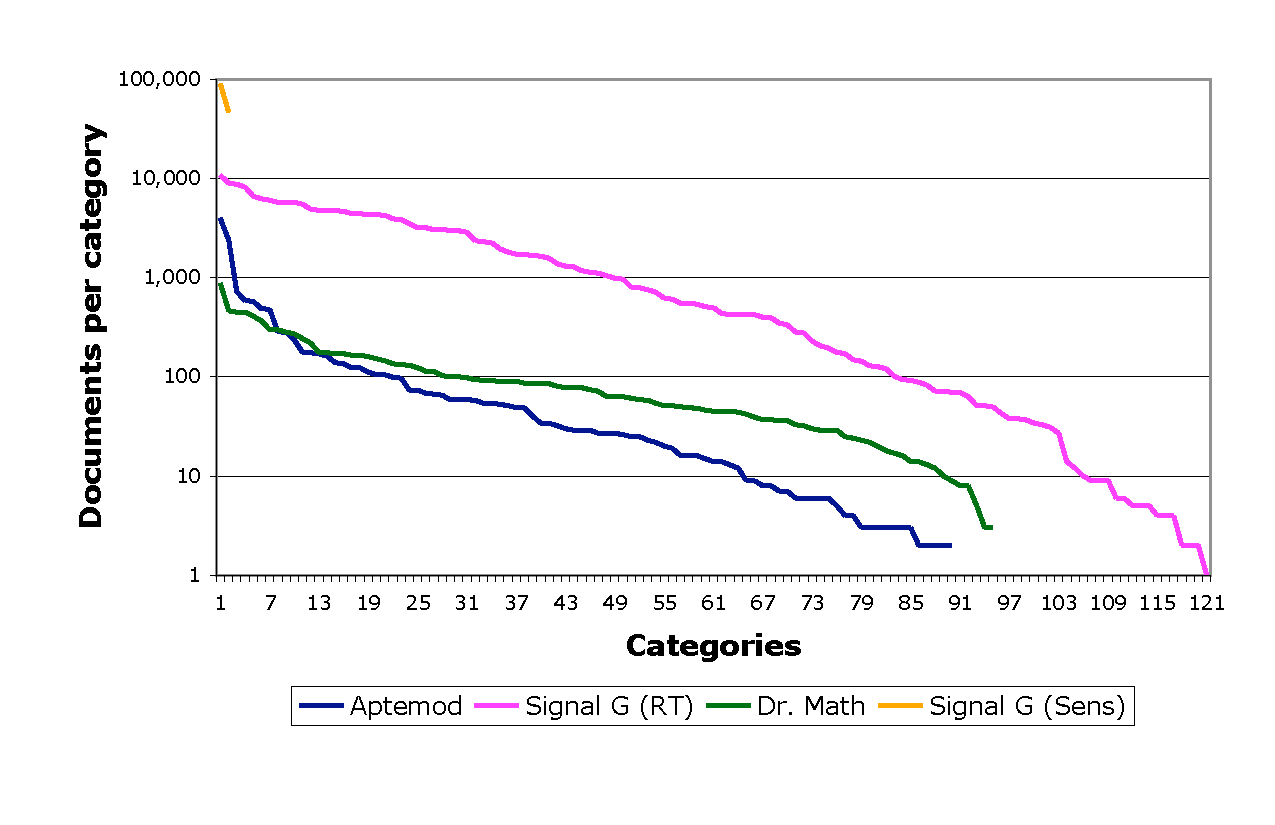
\includegraphics[width=\linewidth]{figures/Corpora-catdist.pdf}
\caption{Category distribution for the four test corpora}
\label{Corpora-catdist}
\end{center}
\end{figure}


\subsection{Dr. Math}

The Dr. Math corpus is a collection of 6,630 English-language messages
sent to the ``Ask Dr. Math'' question-and-answer service for
students.\cite{drmath} Each message has been manually assigned by a
domain expert to one or more categories,
with category names indicating both math topic and grade level,
e.g. ``High School Geometry.''  There are 95 categories in the
category set.  The ontology is generally not
separable into two separate category sets for independent topic and
level categorizations, in part because many topic and level
combinations like ``Elementary School Calculus'' don't exist in the
category scheme.

The 26 MB corpus is divided into a training set with 5,304 documents
and a test set with 1,326 documents.  As with the ApteMod corpus, the
category distribution is skewed, with 13.2\% of the documents in the
most common category and only 0.0452\% (3 documents) in the least
common category.  The average number of categories per document is
1.534, and the average number of documents per category is about 107,
or 1.61\% of the corpus.

The corpus is not available for direct download, but interested
parties may contact the author for details.


\subsection{Signal G (Sensitivity)}

The Signal G corpus consists of 136,630 financial announcement
documents from the Australian Stock Exchange (ASX)\cite{asx:02} issued
between January 4 and December 29, 2000.  Each documents has been
manually categorized by the ASX according to whether it indicates ``market
sensitivity'' or not.  Market sensitivity is a subjective label indicating
whether the given document has potential to affect the issuing
company's share value, trading volume, or other properties on the
exchange.  Every document is a member of either the ``sensitive'' or
``insensitive'' category---this can be viewed as two categories that
partition the corpus, or as a single category that some documents
belong to and others don't.  This discussion assumes the former.

The documents are divided into a training set of 95,525 documents and a
test set of 41,105 documents.  The total size of the corpus is about
342 MB.  Of the 136,630 corpus documents, about 34.0\% are marked as
market sensitive, and the rest are marked as insensitive.

\subsection{Signal G (Report Type)}

The same documents in the previous corpus can also be tagged with a
``report type'' category.  This category indicates the type of
business announcement contained in the document, and may take values
such as ``Notice of Annual General Meeting'' or ``Dividend Books
Closing.''  There are 121 categories in the corpus, with 7.91\%
(10,815 documents) belonging to the most common category, and ten
categories that contain five documents or fewer.  Thus the corpus
exhibits a high skew with respect to this category scheme, similar to
the ApteMod and Dr. Math corpora.

For this corpus with the Report Type labels, the same division between
training and test documents was used as with the Sensitivity labels.



\section{Quality of Categorization}
\label{Quality}

In order to evaluate the quality of the results generated by automatic
categorization systems, researchers usually evaluate the results of
the system on a controlled set of test documents which have manually
been assigned category labels by a human expert.
\cite[pp. 9 \& 37]{sebastiani:02} This is the approach used here,
using the four corpora described in Section \ref{Corpora} as the test
sets.

It should be emphasized that this thesis does not claim to produce any
new results in the area of developing Text Categorization algorithms.
Descriptions of existing algorithms from the TC literature have formed
the basis for developing the \aicat\ framework.  The results presented
here should be considered successful if they align with results
already published in the literature---superior results should not be
expected.

\subsection{Performance Measures}
\label{measures}

Several statistical measures have become standard in the area of
evaluating Text Categorization systems.\cite[p. 33]{sebastiani:02}
Some of the most prevalant are based on the notions of
\emph{precision} and \emph{recall} from the field of Information
Retrieval.\cite{rijsbergen:79} Precision, often denoted by the symbol
$\pi$, measures the probability that a document assigned by the TC
system to a given category actually belongs to that category.
Conversely, recall, denoted by $\rho$, measures the probability that a
document actually belonging to a certain category will be assigned
during testing to that category.\cite[p. 33]{sebastiani:02}

The probabilities mentioned above can be estimated during testing by
comparing how often the TC system's category choices match the correct
categories.  A valuable tool for this analysis is the ``contingency
table,'' which summarizes the results of the experiment for a given
category.  Table \ref{onecat-contingency} shows a contingency table
for the category $c_i$, i.e. any arbitrary category in the
categorization scheme of the corpus.  Here, $A_i$, etc. represent the
number of documents that fall into the given situation, i.e. $A_i$ is
the number of test documents assigned to category $c_i$ by both the
expert and the TC system.

This allows us to estimate $\pi$ and $\rho$, whose true values are
$P(Expert=Y | System=Y)$ and $P(System=Y | Expert=Y)$, respectively,
in terms of the entries in the contingency table.  Since the number of
documents assigned to category $c_i$ by the TC system is $A_i+B_i$,
and the number assigned by the expert is $A_i+C_i$, our estimates for
$\pi$ and $\rho$ are $\frac{A_i}{A_i + B_i}$ and $\frac{A_i}{A_i +
C_i}$, respectively.



\begin{table}
\begin{center}
\begin{tabular}{|c|c|c|c|}
\cline{3-4}
\multicolumn{2}{c|}{} & \multicolumn{2}{c|}{\textbf{Expert choice}} \\
\cline{3-4}
\multicolumn{2}{c|}{} & Yes & No \\
\hline
\textbf{System} & Yes & $A_i$ & $B_i$ \\
\cline{2-4}
\textbf{choice} & No  & $C_i$ & $D_i$ \\
\hline
\end{tabular}
\end{center}
\caption{Contingency table for category $c_i$}
\label{onecat-contingency}
\end{table}


$\pi$ and $\rho$ give valuable information about the performance of a
TC system, but neither provides an isolated rating of the system's
quality.  The reason is that either measure can usually be improved in
a system to the detriment of the other.\cite[p. 35]{sebastiani:02} For
instance, the \emph{trivial acceptor} categorizer, which assigns every
document to every category, will have a perfect $\rho$ score of 1, but
its precision will be unacceptably low on any nontrivial task.

Therefore, a measure that combines $\pi$ and $\rho$ is desirable as an
overall measure of the quality of the TC system.  One such measure is
the $F_\beta$ measure, first introduced to the Information Retrieval
literature by van Rijsbergen \cite[ch. 7]{rijsbergen:79}.  It is
defined by the equation $F_\beta = \frac{(\beta^2 + 1)\pi\rho}{\beta^2
\pi + \rho}$, where $0 \leq \beta \leq \infty$.  The $\beta$ parameter
provides a continuous way to balance between the importance of $\pi$
and $\rho$, with values closer to 0 emphasizing $\pi$, values closer
to $\infty$ emphasizing $\rho$, and a value of 1 balancing the two
measures equally.  Without specific knowledge of an application's
requirements (for instance, whether false positives for a certain
category are more problematic than false negatives), one may presume
that $\pi$ and $\rho$ are equally important, and therefore the
literature often uses $F_1$ as a measure of the quality of a TC system
on a particular category.

${F_1}_i$ may be derived in terms of the entries of the per-category
contingency table as follows:

\begin{equation*}
\begin{split}
{F_1}_i 
 & = \frac{ 2 \pi_i \rho_i}{\pi_i + \rho_i} \\[6pt]
 & = \frac{ \frac{2 {A_i}^2}{(A_i+B_i)(A_i+C_i)} } { \frac{A_i}{A_i+B_i} + \frac{A_i}{A_i+C_i} } \\[6pt]
 & = \frac{ 2 {A_i}^2 }                            { A_i(A_i+C_i) + A_i(A_i+B_i) } \\[6pt]
 & = \frac{ 2 A_i }                                { 2 A_i + B_i + C_i } \\[6pt]
\end{split}
\end{equation*}

Two other measures of categorization quality, \emph{error} and
\emph{accuracy}, are also sometimes encountered in the TC literature.
These are simple measures which can also be defined in terms of the
contingency table in Table \ref{onecat-contingency}: $error =
\frac{B_i+C_i}{A_i+B_i+C_i+D_i)}$, and $accuracy =
\frac{A_i+D_i}{A_i+B_i+C_i+D_i)}$.  In other words, error is the
proportion of the system's decisions that matched the expert's
choices, and accuracy is the proportion that did not.  As summarized
in \cite[p. 34]{sebastiani:02}, these are not always useful measures
of categorization quality, because the \emph{trivial rejector} (a
system that never assigns any documents to any category) will often
have a lower error and higher accuracy than most nontrivial
categorizers.  Nonetheless, error will be measured for the evaluation
tasks here, because it may give insight into the character of the
system's performance.


\subsection{Combining Measures Across Categories}
\label{combining-measures}

Section \ref{measures} introduced several performance measures that
may be defined to evaluate a categorizer on a single category.  In
order to evaluate the categorizer's overall performance on the entire
set of test documents, it is desirable to combine the per-category
scores $\pi_i$, $\rho_i$, and ${F_1}_i$ into overall scores for the
entire category set.

Two methods for doing this are standard in the literature.  The first
is called \emph{micro-averaging}, and sums the terms in the
contingency table for all categories simultaneously rather than in
per-category tables.  In other words, the micro-averaged $\pi$,
$\rho$, and $F_1$, notated $\pi^\mu$, $\rho^\mu$, and $F^\mu_1$, are
defined in terms of the per-category contingency tables by the
following equations.

\begin{equation*}
 \pi^\mu = \frac{\sum_{i=1}^{|C|}{A_i}} {\sum_{i=1}^{|C|}{A_i+B_i}} \qquad
\rho^\mu = \frac{\sum_{i=1}^{|C|}{A_i}} {\sum_{i=1}^{|C|}{A_i+C_i}} \qquad
 F^\mu_1 = \frac{\sum_{i=1}^{|C|}{2 A_i}} {\sum_{i=1}^{|C|}{2 A_i+B_i+C_i}} \qquad
\end{equation*}

Micro-averaging gives equal weight to each categorization decision
made by the system, or equivalently, to each document in the corpus,
regardless of how many categories it belongs to.

An alternative to micro-averaging is \emph{macro-averaging}, in which
the per-category scores $\pi_i$, $\rho_i$, and ${F_1}_i$ are simply
averaged to find the macro-averaged $\pi$, $\rho$, and $F_1$, notated
$\pi^M$, $\rho^M$, and $F^M_1$.  The following equations describe this
procedure.

\begin{equation*}
 \pi^M = \frac{\sum_{i=1}^{|C|}{\pi_i}}   {|C|} \qquad
\rho^M = \frac{\sum_{i=1}^{|C|}{\rho_i}}  {|C|} \qquad
 F^M_1 = \frac{\sum_{i=1}^{|C|}{{F_1}_i}} {|C|} \qquad
\end{equation*}

Macro-averaging gives equal weight to each category in the corpus,
regardless of how many documents it contains.  Thus it provides a
good counterpart to micro-averaging; macro-averaging will place more
emphasis on rare categories than micro-averaging, so reporting both
scores is typically useful to evaluate the system as a whole.

Note that the error and accuracy measures are unaffected by micro-
vs. macro-averaging, as shown in the following derivation.  This uses
the observation that $A_i+B_i+C_i+D_i = |\test|$, a consequence of the
fact that exactly one of the terms on the left side will be
incremented with each decision about whether a document from the test
set belongs to $c_i$ or not.

\begin{equation*}
\begin{split}
error^M
 & = \frac{\sum_{i=1}^{|\cats|}{error_i}}  {|\cats|} \\[6pt]
 & = \frac{\sum_{i=1}^{|\cats|}{ \frac{B_i+C_i}{A_i+B_i+C_i+D_i} }} { \sum_{i=1}^{|\cats|}{1} } \\[6pt]
 & = \frac{\sum_{i=1}^{|\cats|}{ \frac{B_i+C_i}{|\test|} }}         { \sum_{i=1}^{|\cats|}{1} } \\[6pt]
 & = \frac{\sum_{i=1}^{|\cats|}{B_i+C_i}}                           { \sum_{i=1}^{|\cats|}{|\test|} } \\[6pt]
 & = \frac{\sum_{i=1}^{|\cats|}{B_i+C_i}}                           { \sum_{i=1}^{|\cats|}{A_i+B_i+C_i+D_i} } \\[6pt]
 & = error^\mu
\end{split}
\end{equation*}


\subsection{Results}

Using the measures defined in Sections \ref{measures} and
\ref{combining-measures}, categorization experiments were performed on
each of the four corpora described in Section \ref{Corpora}.  Several
experimental parameters (e.g. category membership thresholds) can be
set for each experiment; for the ApteMod corpus these were set to
match the parameters used in \cite{yang:99}, where known.  For the
other corpora they were optimized to provide the
best performance on the test set---in this sense, the test set might
be thought of more correctly as a validation set, because in a strict
testing environment the performance on the test set should not
influence training parameters.  This methodology was adopted because
it more closely matches the procedure that would be used when building
an application, in which the true test set may consist of documents
not yet posessed by the developer, i.e. the set of target documents
in the application domain.  This is the evaluation method used in
several studies in the literature, such as \cite{joachims:98}.

Where a baseline score is given in the results, this refers to a
simple probabilistic categorizer that assigns categories to each
document, weighting the probability of assignment by the frequency of
each category in the training set.  For instance, if a certain
category was present in 40\% of the training documents, any document
in the test set would have a probability of 0.4 of being assigned to
that category by the baseline categorizer.  

\subsubsection{ApteMod}

Table \ref{aptemod-results} summarizes the results of three different
machine learning methods in \aicat\ as compared with the baseline
categorizer described above.  Table \ref{aptemod-yang} gives similar
scores from a well-known comparitive study of common categorization
algorithms.\cite{yang:99} Where possible, the present study has
attempted to duplicate the findings in \cite{yang:99}, though in some
cases there is not enough information to duplicate the findings
exactly, and in some cases the \aicat\ framework lacks certain
features mentioned in \cite{yang:99}.  These differences will be
discussed below.

\begin{table}
\begin{center}
\begin{tabular}{|r c c c c c c c|}
\hline
%              maR       maP       maF1      miR          miP         miF1
method    & $\rho^M$ & $\pi^M$ & $F_1^M$ & $\rho^\mu$ & $\pi^\mu$ & $F_1^\mu$ &   error \\
\hline
NB        &   .3659  &  .4969  &  .3959  &  .7238     &  .8514    &  .7824    &  .00555 \\
SVM       &   .0868  &  .3727  &  .1239  &  .5254     &  .9106    &  .6663    &  .00725 \\
kNN       &   .2655  &  .3856  &  .2903  &  .7650     &  .7975    &  .7809    &  .00591 \\
Baseline  &   .0135  &  .0142  &  .0137  &  .1645     &  .1664    &  .1654    &  .02287 \\
\hline
\end{tabular}
\end{center}
\caption{Results of \aicat\ on ApteMod corpus}
\label{aptemod-results}
\end{table}

\begin{table}
\begin{center}
\begin{tabular}{|r c c c c c c c|}
\hline
method & $\rho^M$ & $\pi^M$ & $F_1^M$ & $\rho^\mu$ & $\pi^\mu$ & $F_1^\mu$ & error \\
\hline
NB  & ? & ? & .3886 & .7688 & .8245 & .7956 & .00544 \\
SVM & ? & ? & .5251 & .8120 & .9137 & .8599 & .00365 \\
kNN & ? & ? & .5242 & .8339 & .8807 & .8567 & .00385 \\
\hline
\end{tabular}
\end{center}
\caption{Results from \cite{yang:99} on ApteMod corpus}
\label{aptemod-yang}
\end{table}

In the case of the \naive\ Bayes categorizer (NB), the results match
\cite{yang:99} closely, with a slightly greater $F_1^M$ and a slightly
smaller $F_1^\mu$. (XXX - not sure whether I can say that the
differences are statistically insignificant or not.  Need to
understand Yang's stats tests better?)  To match the experimental
settings in \cite{yang:99}, the size of the feature-set was set to
2000.

For the Support Vector Machine categorizer (SVM), the performance is
significantly worse than the findings in \cite{yang:99}.  The reasons
for this are not clear---\aicat\ currently uses an SVM implementation
based on the \texttt{libsvm} C library \cite{libsvm}, whereas
\cite{yang:99} used $SVM^{light}$ as its
implementation\cite{joachims:99a}, and there may be major differences
in the behavior of these two libraries.  Since the macro-averaged scores are
particularly bad, it may be inferred that \cite{libsvm} is not
performing well on rare categories.  In both studies, a linear SVM
kernel was used, and 10,000 features were considered when building the
categorization model.

One possible reason for the poor performance of the SVM categorizer is
that for both micro- and macro-averaged scores, $\pi$ is much larger
than $\rho$, indicating that this situation could be balanced by
choosing more appropriate category membership thresholds.  However,
\texttt{libsvm} doesn't seem to allow tuning of these thresholds, so a
remedy for this situation isn't clear.

For the k-Nearest-Neighbor categorizer (kNN), $F_1^\mu$ results are comparable
with NB, but no scores are as good as the kNN results in \cite{yang:99}.
The major difference between the two implementations is that the
implementation in \cite{yang:99} finds per-category membership
thresholds by optimizing performance on a validation set, while the
implementation in \aicat\ uses a single membership threshold for all
categories, settable by the user.  In this experiment the threshold
was set to 0.1, a value which is not meaningful in itself, but which
seemed to give the best performance.  Note, that the macro-averaged
precision is higher than recall, but the micro-averaged recall is
higher than precision, indicating that it is not possible to
simultaneously find the optimal threshold for both rare and common
categories.  Thus using individual thresholds for each category should
increase $F_1$ scores if optimized properly.  The $k$ parameter
in this experiment
(indicating the number of similar documents to consider when
categorizing) was set to 45, and the number of features considered was
set to 2415, both to match the values used in \cite{yang:99}.

The kNN implementation in \aicat\ is fairly new, and is an adaptation
of work by another researcher.  The ability to optimize per-category
thresholds is considered a useful future addition to the framework,
and will be added soon.

For all three categorizers, the \param{tfidf\_weighting} parameter was set to
\texttt{xfx}, indicating that words are weighted by the logarithm of
their inverse document frequency.  This is the same setting used in
\cite{yang:99}.  One other possible difference between \cite{yang:99}
and the current experiment is that \cite{yang:99} used either a
$\chi^2$ or \emph{information gain} criterion (it is not clear which
criterion was used with which categorizer) for feature selection,
while \emph{document frequency} was used here.  This should not be a
major factor in the results, as document frequency has been shown to
produce results competitive with other feature selection methods on
this corpus. \cite{yang:97}



\subsubsection{Dr. Math}

Table \ref{drmath-results} shows the categorization performance of
\aicat\ on the Dr. Math corpus.  Note that the baseline micro-averaged
scores are much lower than on the ApteMod corpus (Table
\ref{aptemod-results}), indicating that this may be a more difficult
categorization task simply because the category distribution is
flatter than in ApteMod (Figure \ref{Corpora-catdist}).


\begin{table}
\begin{center}
\begin{tabular}{|r c c c c c c c|}
\hline
%              maR       maP       maF1      miR          miP         miF1
method    & $\rho^M$ & $\pi^M$ & $F_1^M$ & $\rho^\mu$ & $\pi^\mu$ & $F_1^\mu$ &   error \\
\hline
NB        &   .2338  &  .2677  &  .2358  &  .3766     &  .3542    &  .3651    &  .0215  \\
SVM       &   .3333  &  .1562  &  .1946  &  .4211     &  .2273    &  .2952    &  .0330  \\
kNN       &   .2372  &  .2824  &  .2154  &  .3607     &  .3572    &  .3590    &  .0212  \\
Baseline  &   .0156  &  .0176  &  .0161  &  .0406     &  .0421    &  .0413    &  .0310  \\
\hline
\end{tabular}
\end{center}
\caption{Results of \aicat\ on Dr. Math corpus}
\label{drmath-results}
\end{table}

Because no other TC study has been done on the Dr. Math corpus, not
much can be said about the comparitive results of the \aicat\
framework.  However, the noteworthy points will be discussed below.

Using the \naive\ Bayes categorizer, the $F_1$ scores are about 0.24
when macro-averaged and 0.37 when micro-averaged.  This is not as
dramatic a difference as seen on the ApteMod corpus, where the
micro-averaged scores are approximately double the macro-averaged
scores.  In this experiment, the number of features considered was set
to 20% of the training corpus, or 1764 features, though varying this
parameter between 1500 and 3000 seemed to produce similar results.

Using the SVM categorizer, $F_1$ scores were again worse than with NB,
but in this case the recall with SVM was higher than the
precision---the opposite of the situation on the ApteMod corpus.
Again, a mechanism for trading off $\rho$ and $\pi$ would be
desirable.  The best scores with SVM were obtained when using no
feature selection at all, i.e. using all 8824 features when building
the SVM models.  This is an indication of SVM's robustness to noise in
the data sets it considers.

With the kNN categorizer, results were competitive with the NB
categorizer.  Note that $F_1^M$ for kNN is lower than each of $\rho^M$
and $\pi^M$---this somewhat counterintuitive situation, unique to
macro-averaging, can arise when the per-category scores $\rho_i$ are
sometimes greater than $\pi_i$ and sometimes less than $\pi_i$.  The
best results for this experiment were found when using a feature set
with 3000 features and $k=15$.


\subsubsection{Signal G (Sensitivity)}

The results of testing \aicat\ on the Signal G (Sensitivity) corpus
have been previously described in detail in \cite{calvo:02}, but the
important points will be discussed here.  Table
\ref{signalg-sens-results} summarizes the findings.  Because there are
only two categories in this corpus, the scores for the baseline
categorizer are much higher than in the other corpora.

The Signal G corpus contains many more documents than the other
corpora, and this caused some issues for categorization.

For the NB, SVM, and kNN categorizers, a feature set with 5000 terms
was used, which is larger than the feature set used in
\cite{calvo:02}.  No real attempt was made to optimize the size of the
feature set, but it was felt that a larger feature set might give
better performance, and (XXX - this was/was not the case).

The \naive\ Bayes categorizer was


\begin{table}
\begin{center}
\begin{tabular}{|r c c c c c c c|}
\hline
%              maR       maP       maF1      miR          miP         miF1
method    & $\rho^M$ & $\pi^M$ & $F_1^M$ & $\rho^\mu$ & $\pi^\mu$ & $F_1^\mu$ &   error \\
\hline
NB        &   .90    &  .90    &  .90    &  .84       &  .83      &  .83      &         \\
SVM       &   .79    &  .80    &  .80    &  .82       &  .82      &  .82      &         \\
kNN       \\
Baseline  &   .5018  &  .4988  &  .5003  &  .5544     &  .5511    &  .5527    &  .4486  \\
\hline
\end{tabular}
\end{center}
\caption{Results of \aicat\ on Signal G (Sensitivity) corpus}
\label{signalg-sens-results}
\end{table}


\subsubsection{Signal G (Report Type)}

The results of testing \aicat\ on the Signal G (Sensitivity) corpus
have also been previously described in \cite{calvo:02}.  Table
\ref{signalg-rt-results} summarizes the present findings.

\begin{table}
\begin{center}
\begin{tabular}{|r c c c c c c c|}
\hline
%              maR       maP       maF1      miR          miP         miF1
method    & $\rho^M$ & $\pi^M$ & $F_1^M$ & $\rho^\mu$ & $\pi^\mu$ & $F_1^\mu$ &   error \\
\hline
NB        \\
SVM       \\
kNN       \\
Baseline  &   .0452  &  .0286  &  .0286  &  .0356     &  .0354    &  .0355    &  .0234  \\
\hline
\end{tabular}
\end{center}
\caption{Results of \aicat\ on Signal G (Report Type) corpus}
\label{signalg-rt-results}
\end{table}

\section{Efficiency}
\label{Efficiency}

\section{Applications}
\label{Applications}



\chapter{Conclusion}


\appendix
\addcontentsline{toc}{chapter}{Appendix A: A Framework for Text Categorization}
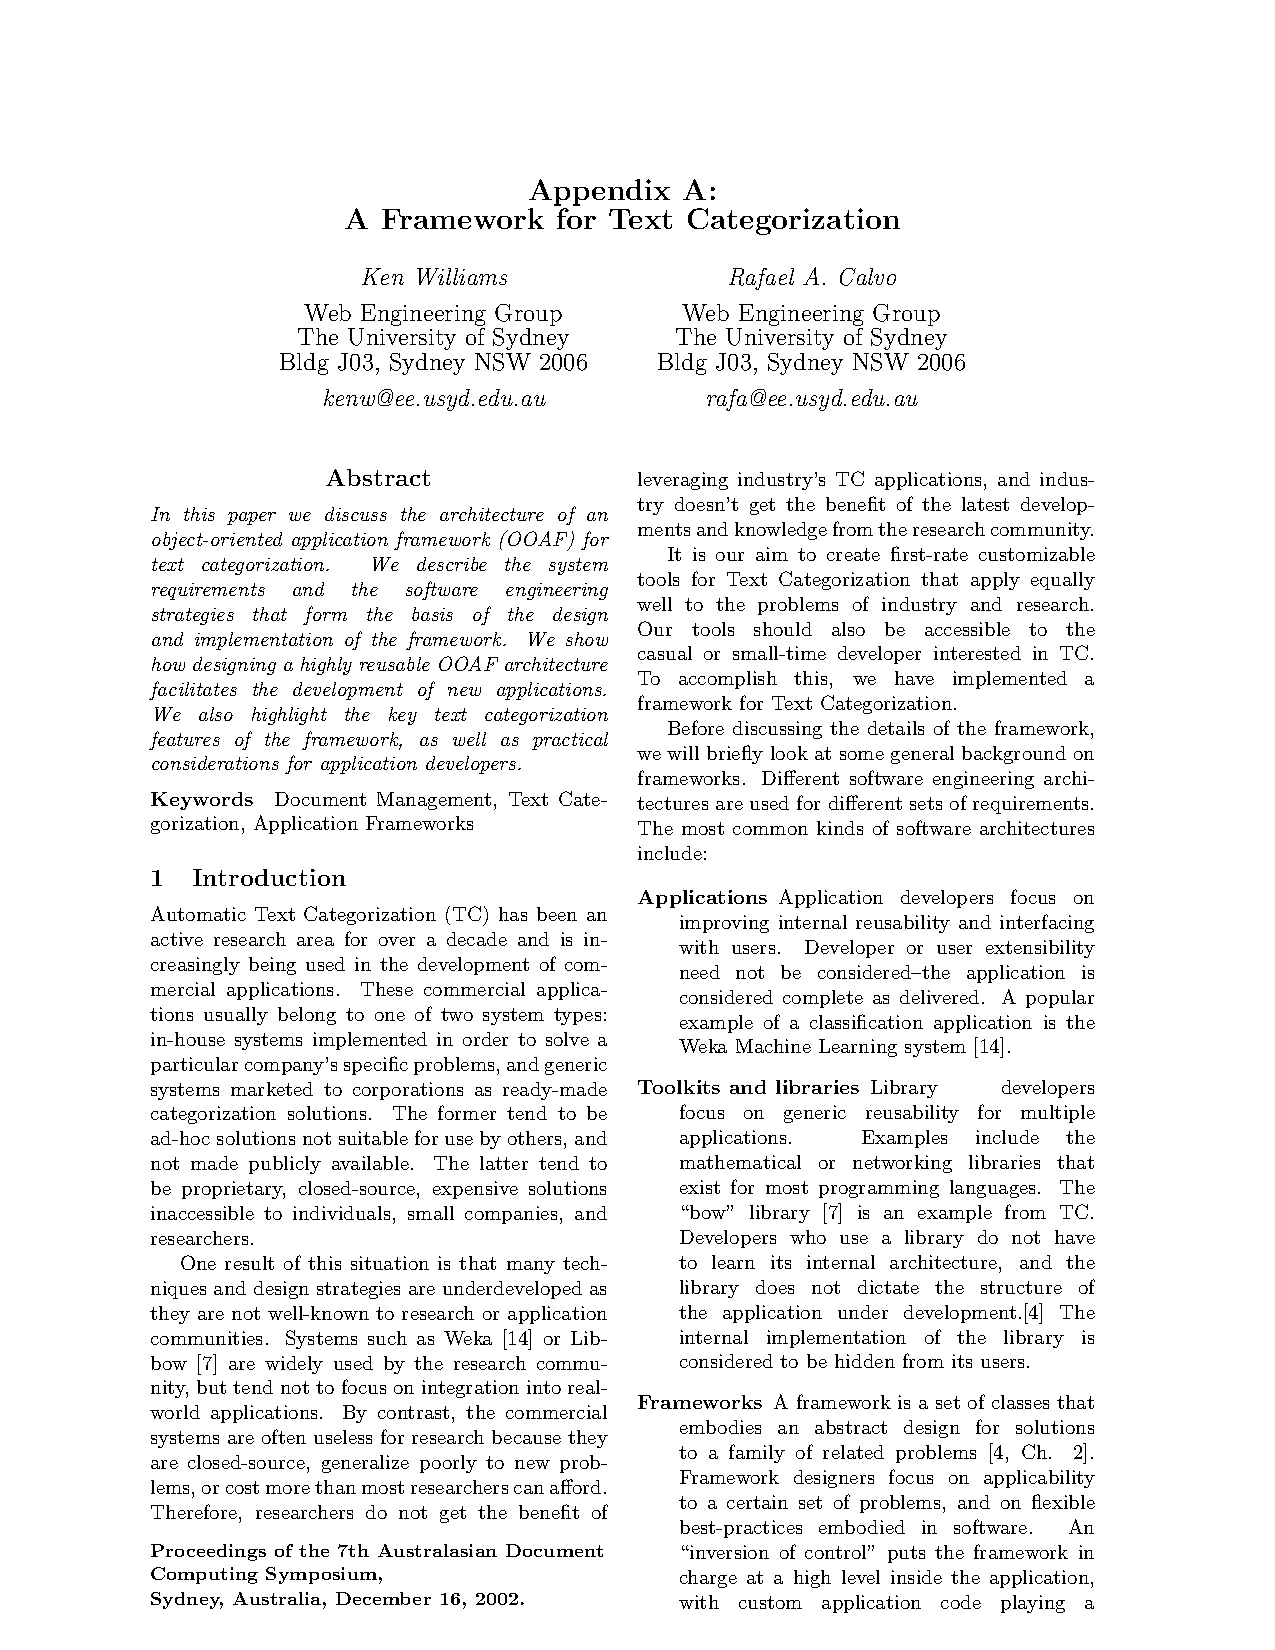
\includepdf[pages=-]{ap01.pdf}
\addcontentsline{toc}{chapter}{Appendix B: Automatic Categorization of Announcements \\
                               on the Australian Stock Exchange}
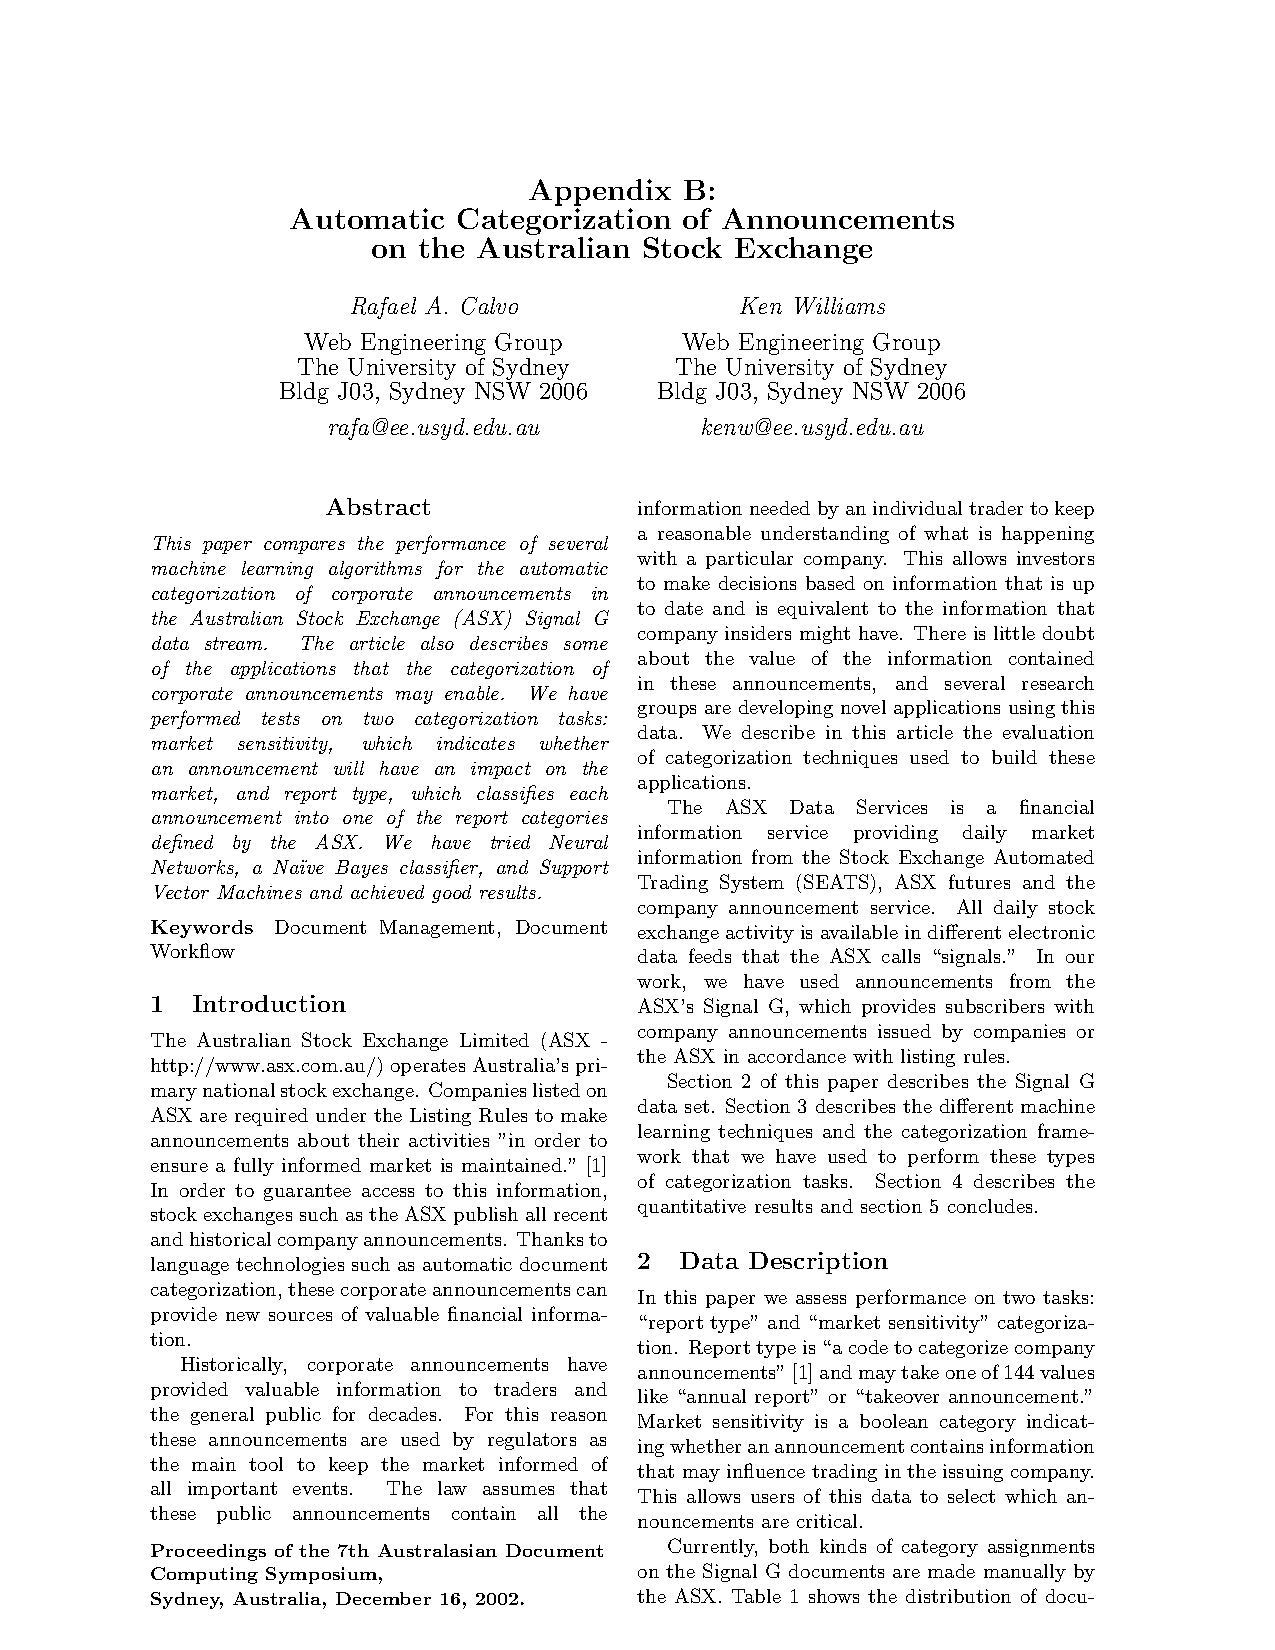
\includepdf[pages=-]{ap02.pdf}
\addcontentsline{toc}{chapter}{Appendix C: Automatic Categorization of Questions \\
                               for a Mathematics Education Service}
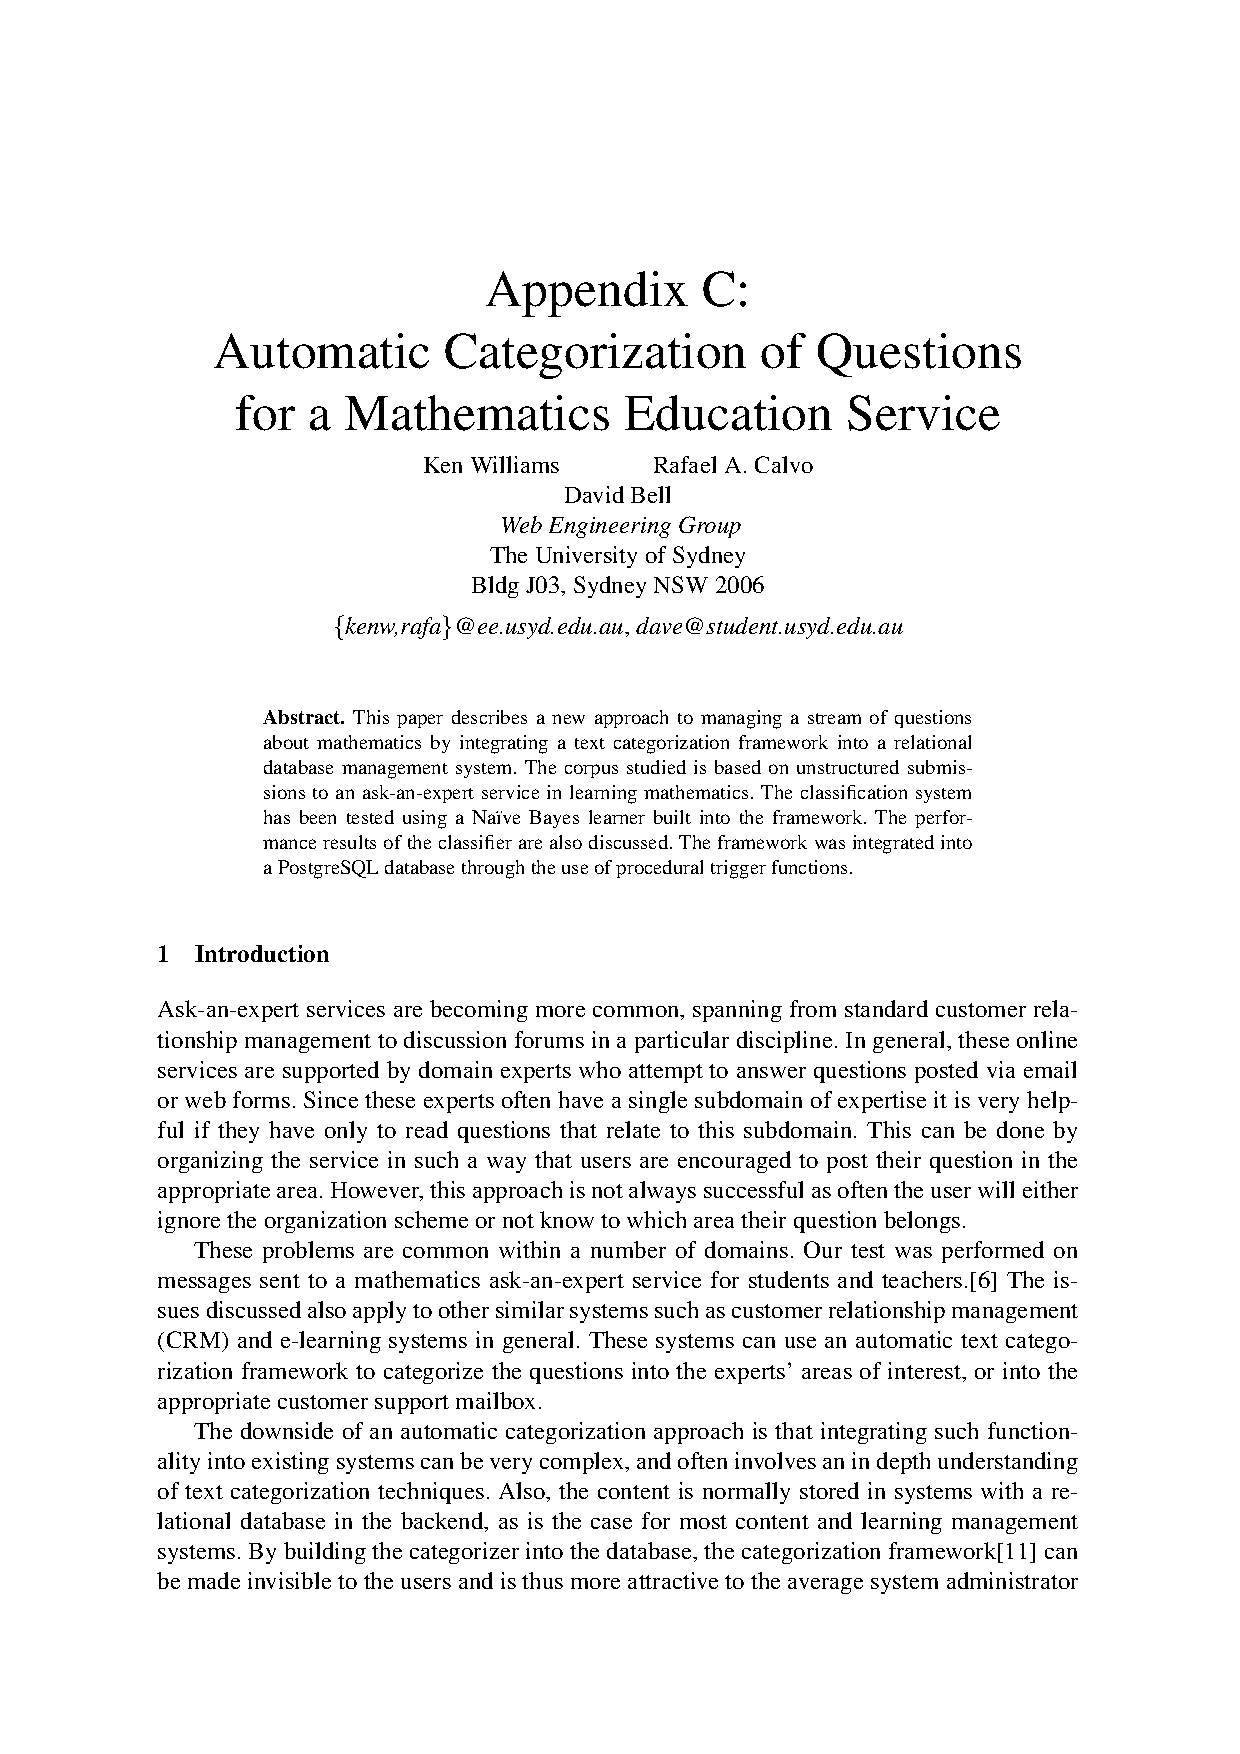
\includepdf[pages=-]{ap03.pdf}

\backmatter
\addcontentsline{toc}{chapter}{Bibliography}
\bibliographystyle{plain}
\bibliography{TC-references}

\end{document}
